\chapter{Performance of the Particle Flow algorithm in data/MC comparison}

To study the performance of the Particle Flow algorithm in Run 2 data/Monte Carlo comparison a  $Z \rightarrow \mu \mu$ decay has been chosen. The used dataset was wildcard and wildcard was used for the Monte Carlo. The chapter explains the choice of decay and gives a overview over the event selection before showing a summary of performance plots. 

\section{The $Z \rightarrow \mu \mu$ decay}
\begin{figure}[h]\centering
\begin{fmffile}{ztomumu}
\begin{fmfgraph*}(50,30) \fmfpen{thin}
  \fmfleft{i1} \fmfright{o1,o2}
  \fmf{wiggly, label=$Z$}{i1,v1}
  \fmf{fermion, label=$\mu$}{v1,o2}
  \fmf{fermion, label=$\overline{\mu}$}{v1,o1}
  \end{fmfgraph*}
\end{fmffile}
\caption{Decay of a Z-Boson to two muons}
\label{decay}
\end{figure}


For this thesis $Z\rightarrow \mu \mu$ events were used. The deay channel of a $Z$ boson into a muon and a antimuon has a crossection of \num{3.366 +- 0.007} \cite{pdg}. The event was chosen for this analysis because the Z boson is very easy to trigger on and it allows a very clear event selection. Furthermore the event has exactly one recoiling jet that analysis can be performed on. 

\section{Event selection}
The criteria for the event selection were no good electrons and exactly two good muons, with opposite charge where good means that the particle passed all selection filters itself. The muons are required to have a transversal momentum greater than \SI{25}{\GeV}. Furthermore the muons are restricted to a central $\eta$ region being $|\eta|<2.4$.

Furthermore a jet is required to have a transversal momentum greater than \SI{20}{\GeV} and is required to be recoiling to the reconstructed Z giving the selection criteria $|\phi_{jet}-\phi_Z|<(\pi - \num0.4)$.
The region of pseudorapidity is limited to  $|\eta|<2.5$ to ake into account the the inner tracking detector covers only this region.

Figure one shows the number of events selected. 

\section{Kinematic variables of muons and jets}

After selecting proper $Z \rightarrow \mu \mu$ events the agreement between data and MC has been studied for the selected objects. This section summarizes the kinematic variables of the muons and the chosen recoiling jet.

Figure \ref{fig:muons} shows the kinematic variables of the muons. For $pT<\SI{100}{\GeV}$ and $e<\SI{300}{\GeV}$ the agreement between data and Monte Carlo for momentum and energy is very good. In greater momentum regions the agreement worsens significantly. This might have its reason in insufficient statistics. For $\eta$ and $\phi$ the agreement is quite good.

The recoiling jet properties are shown in figure \ref{fig:reoilingjet}. The agreement for $pT$ and energy are rather bad for the jets especially in high energy regions but even in low $pT$ and energy regions the agreement is far worse than expected.
The angular agreement looks better except for $|\eta|>2.5$ which is outside the tracker region and could be excluded for Particle Flow performance analysis.



\begin{figure}[h]
\centering
\begin{subfigure}[b]{0.5\figwidth}
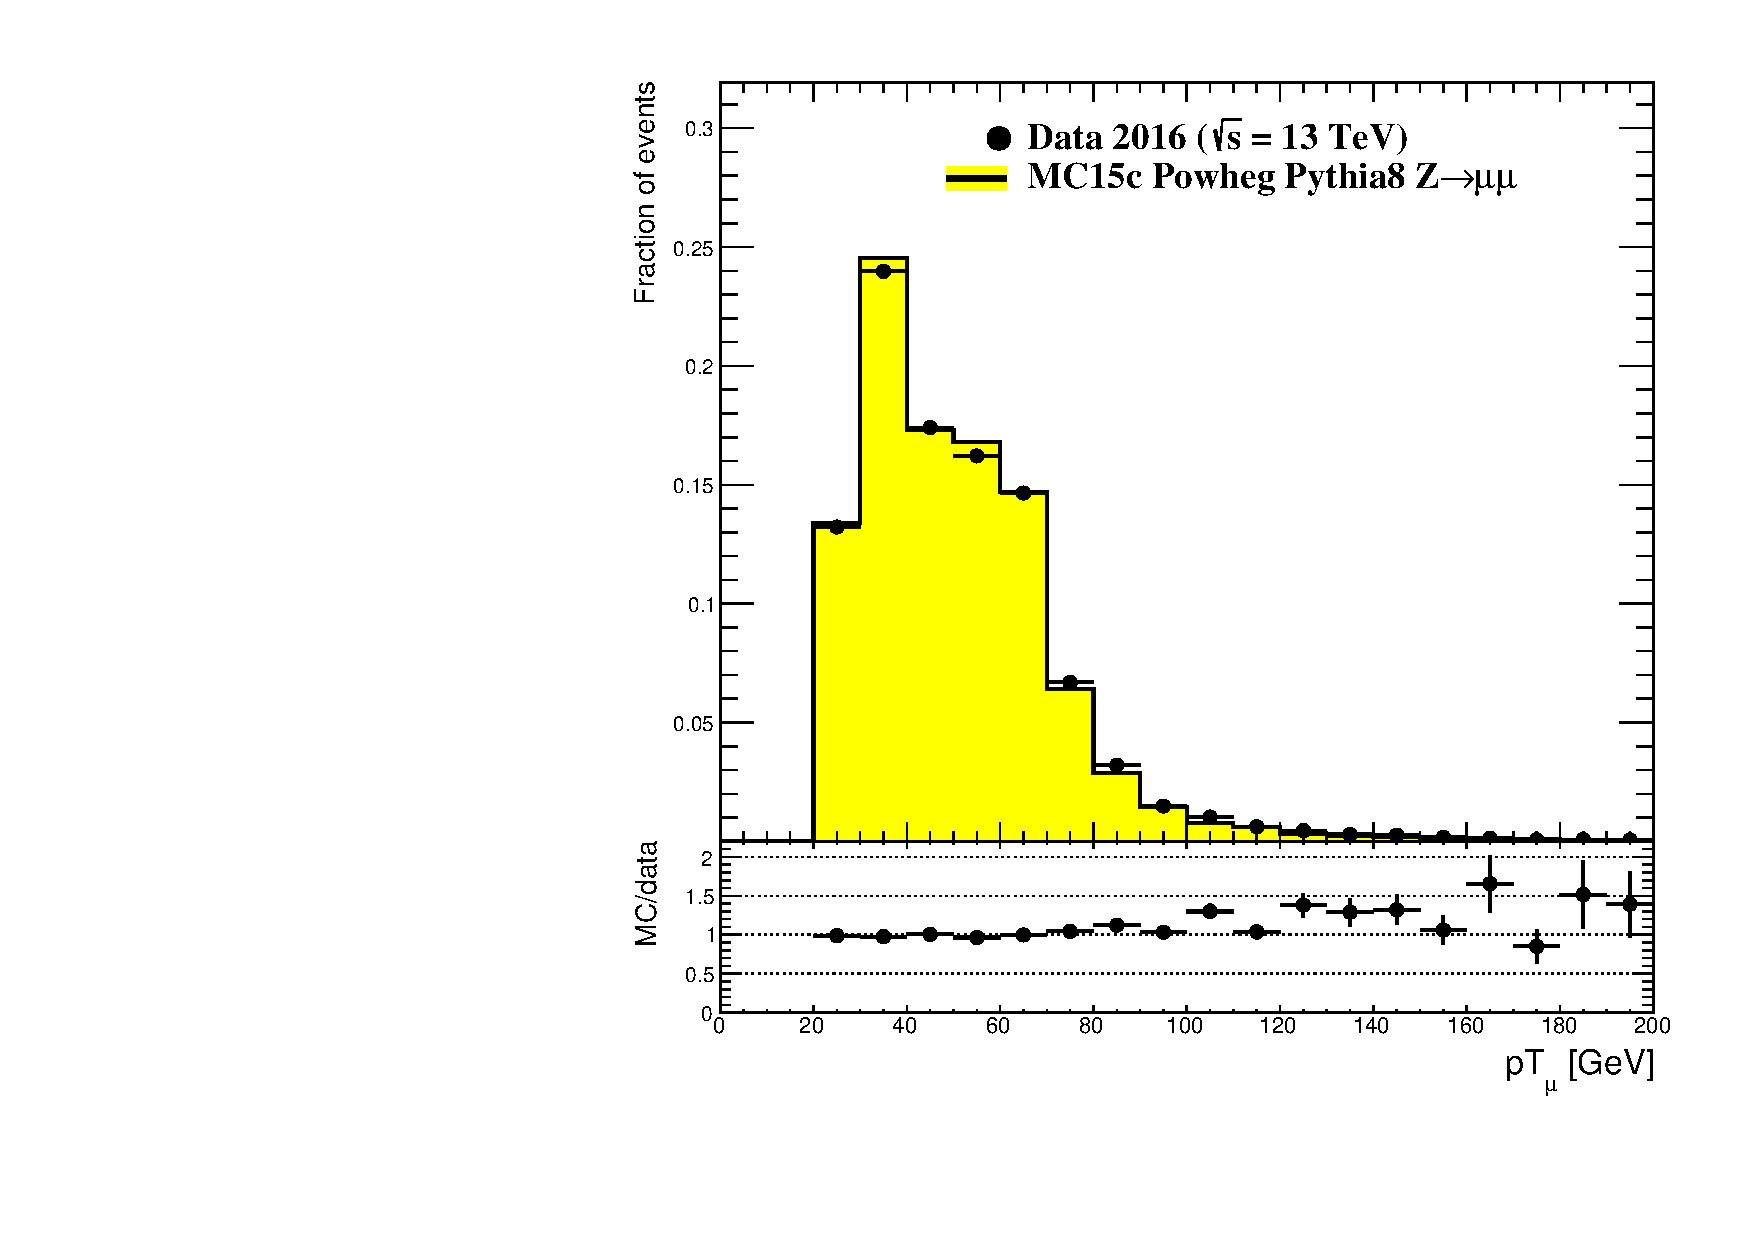
\includegraphics[width=0.53\figwidth]{muon_ptratio}
\caption[Transversal momentum of the muons]{$pT_{\mu}$}
\label{fig:muonpt}
\end{subfigure}
\quad
\begin{subfigure}[b]{0.5\figwidth}
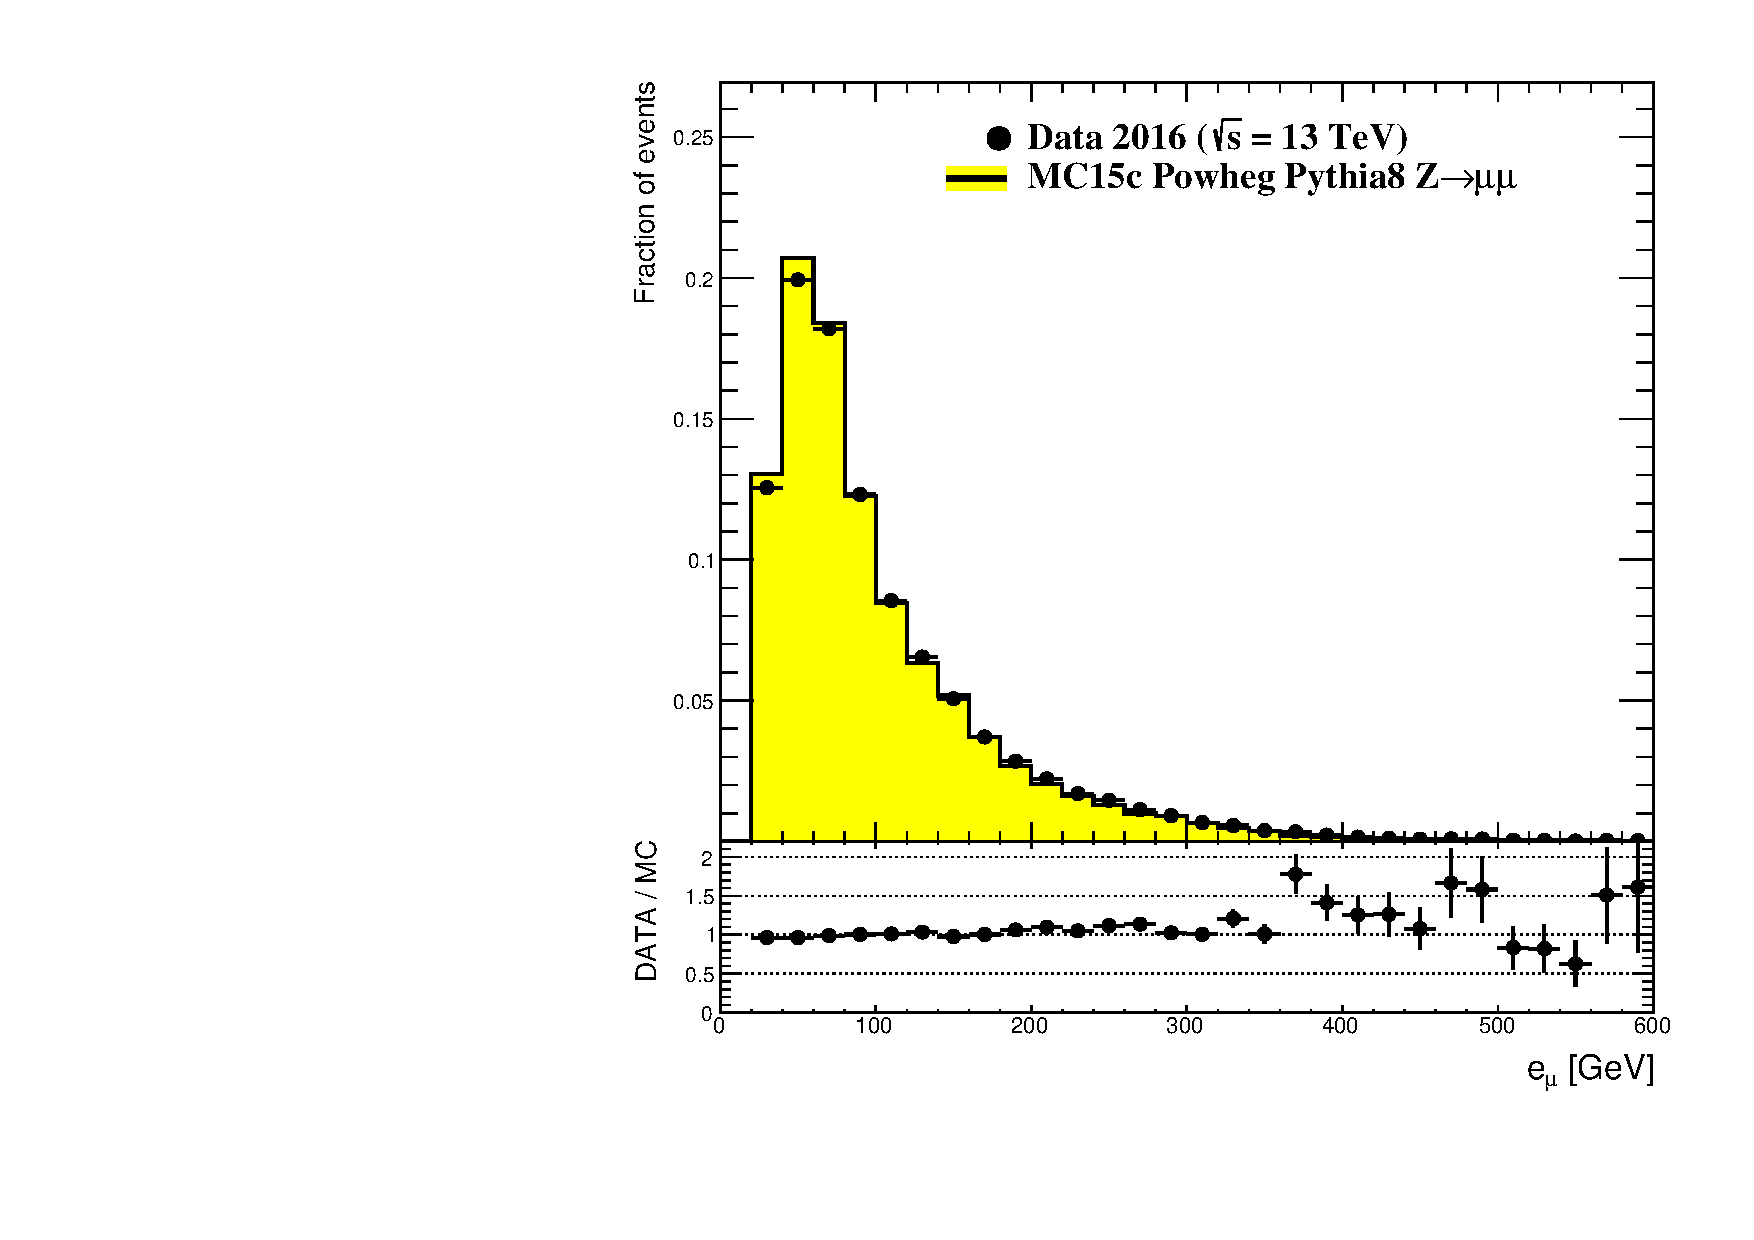
\includegraphics[width=0.53\figwidth]{muon_eratio}
\caption[Energy of the muons]{$e_{\mu}$}
\label{fig:muone}
\end{subfigure}
\end{figure}


\begin{figure}[h]
\centering
\begin{subfigure}[b]{0.5\figwidth}
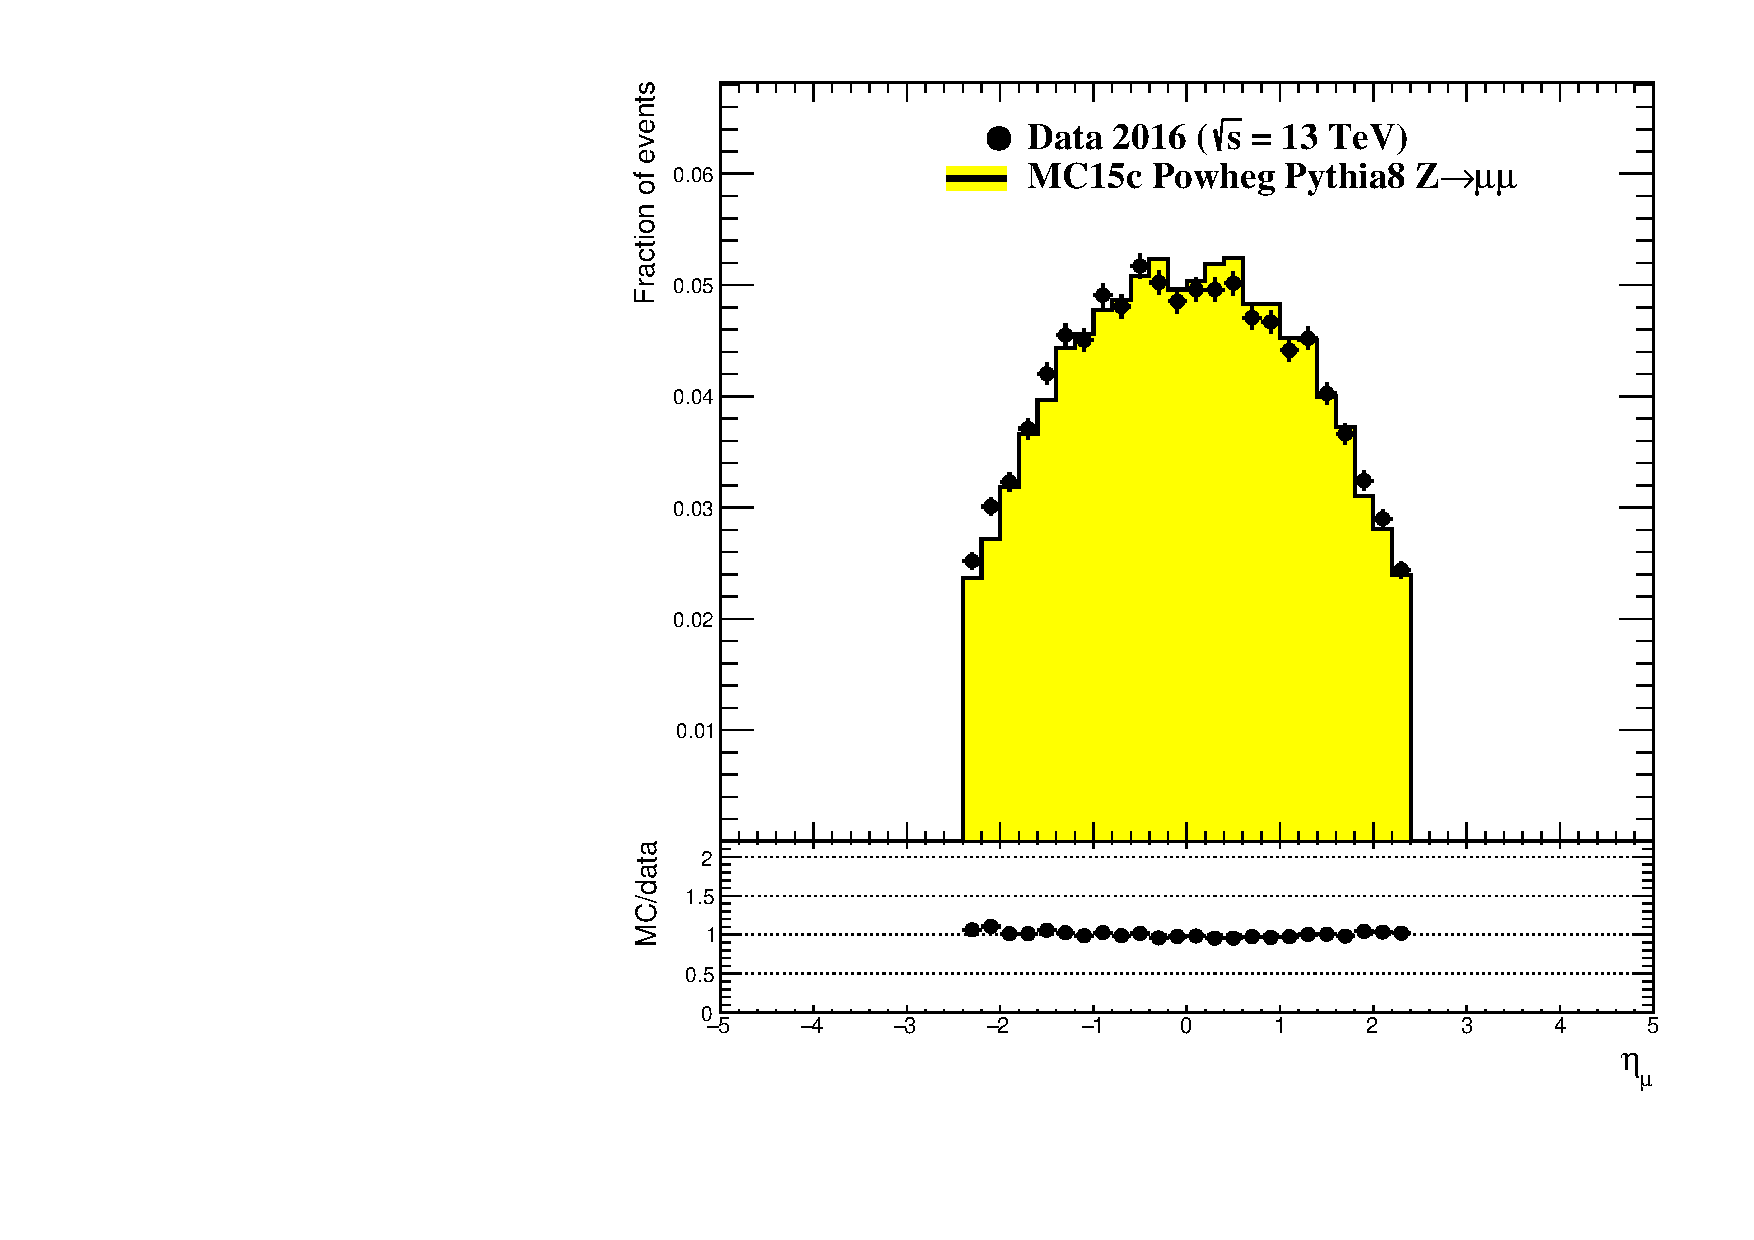
\includegraphics[width=0.53\figwidth]{muon_etaratio}
\caption[$\eta$ of the muons]{$\eta_{\mu}$}
\label{fig:muoneta}
\end{subfigure}
\quad
\begin{subfigure}[b]{0.5\figwidth}
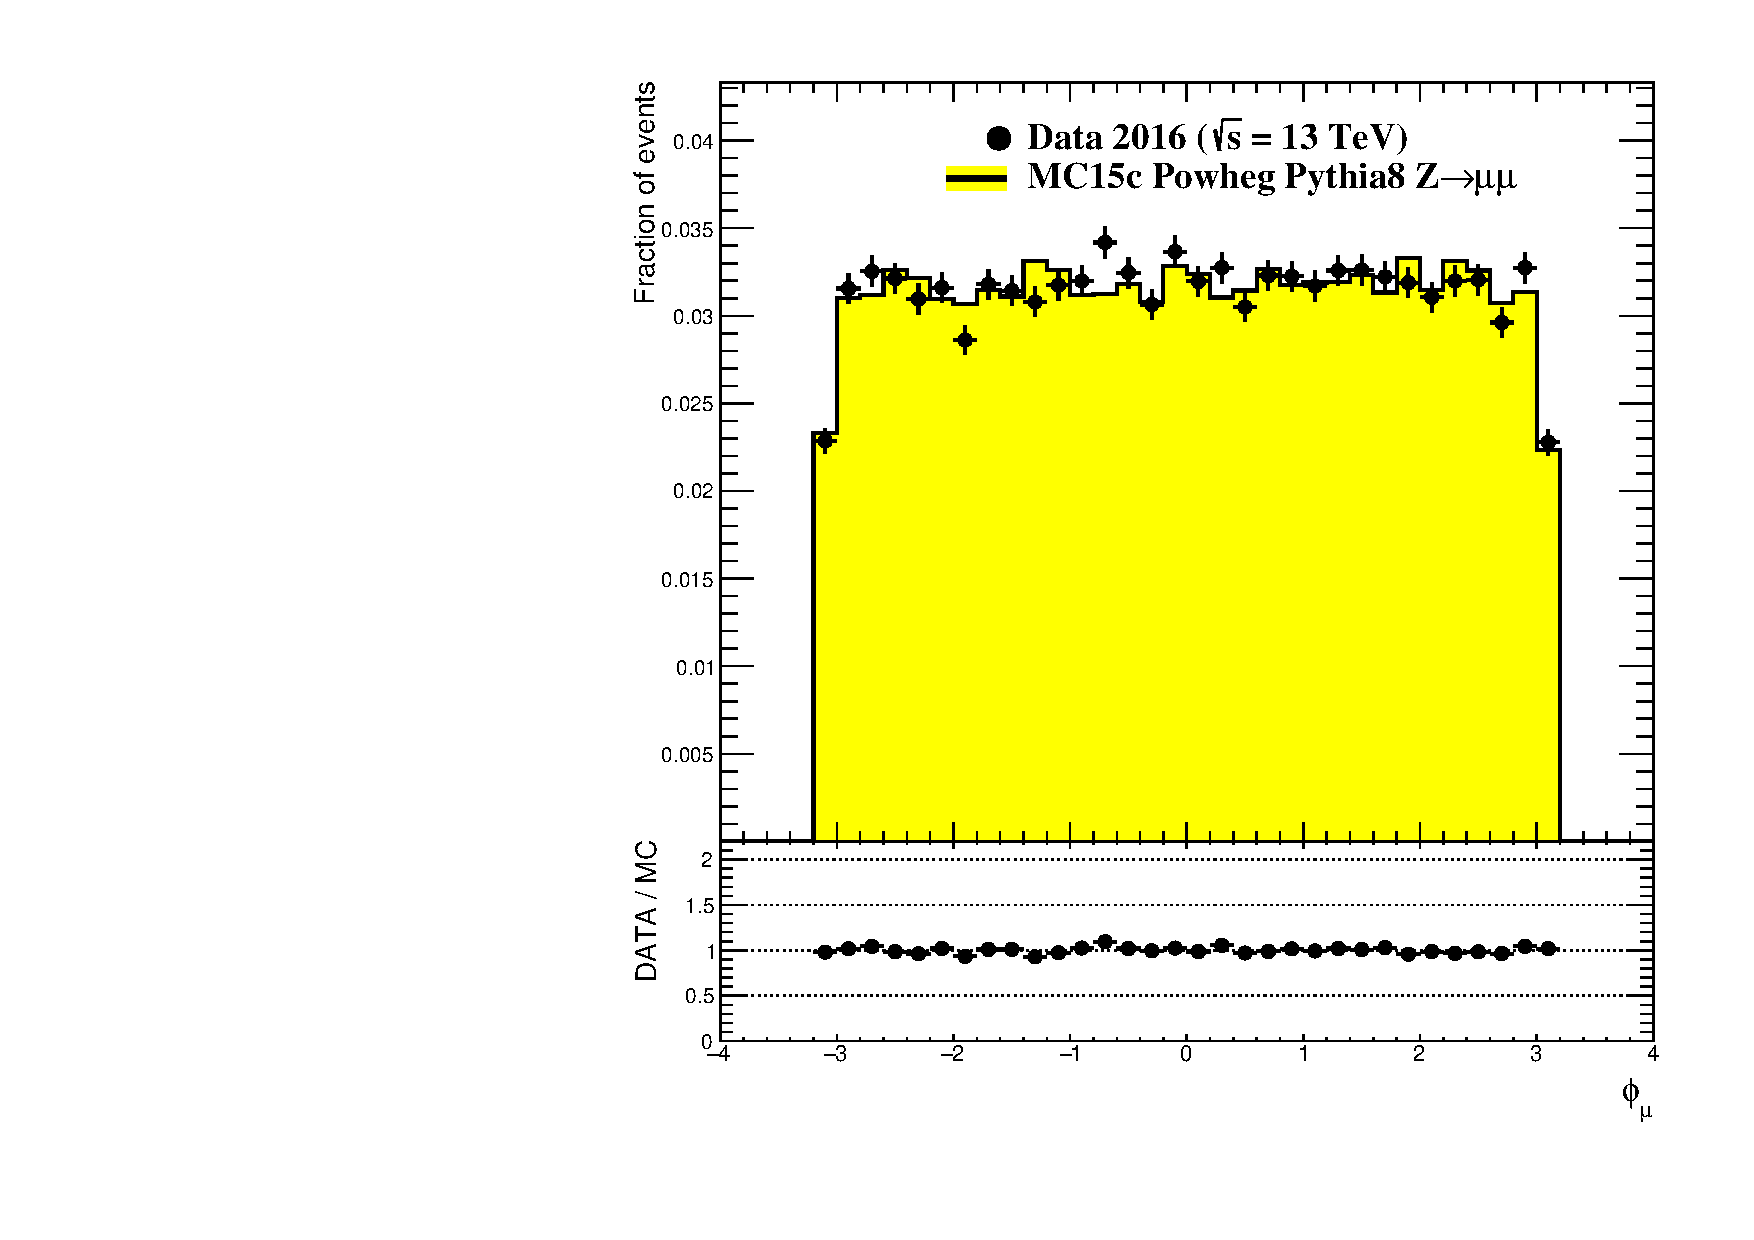
\includegraphics[width=0.53\figwidth]{muon_phiratio}
\caption[$\phi$ of the muons]{$\phi_{\mu}$}
\label{fig:muonphi}
\end{subfigure}
\caption{Properties of the two muons. The histograms are normalized. The distributions shown are: \ref{fig:muonpt} the transversal momentum of the muons; \ref{fig:muone} the muons' energy; \ref{fig:muoneta} the muons' $\eta$ and \ref{fig:muonphi} the muons' $\phi$}
\label{fig:muons}
\end{figure}


\begin{figure}[h]
\centering
\begin{subfigure}[b]{0.5\figwidth}
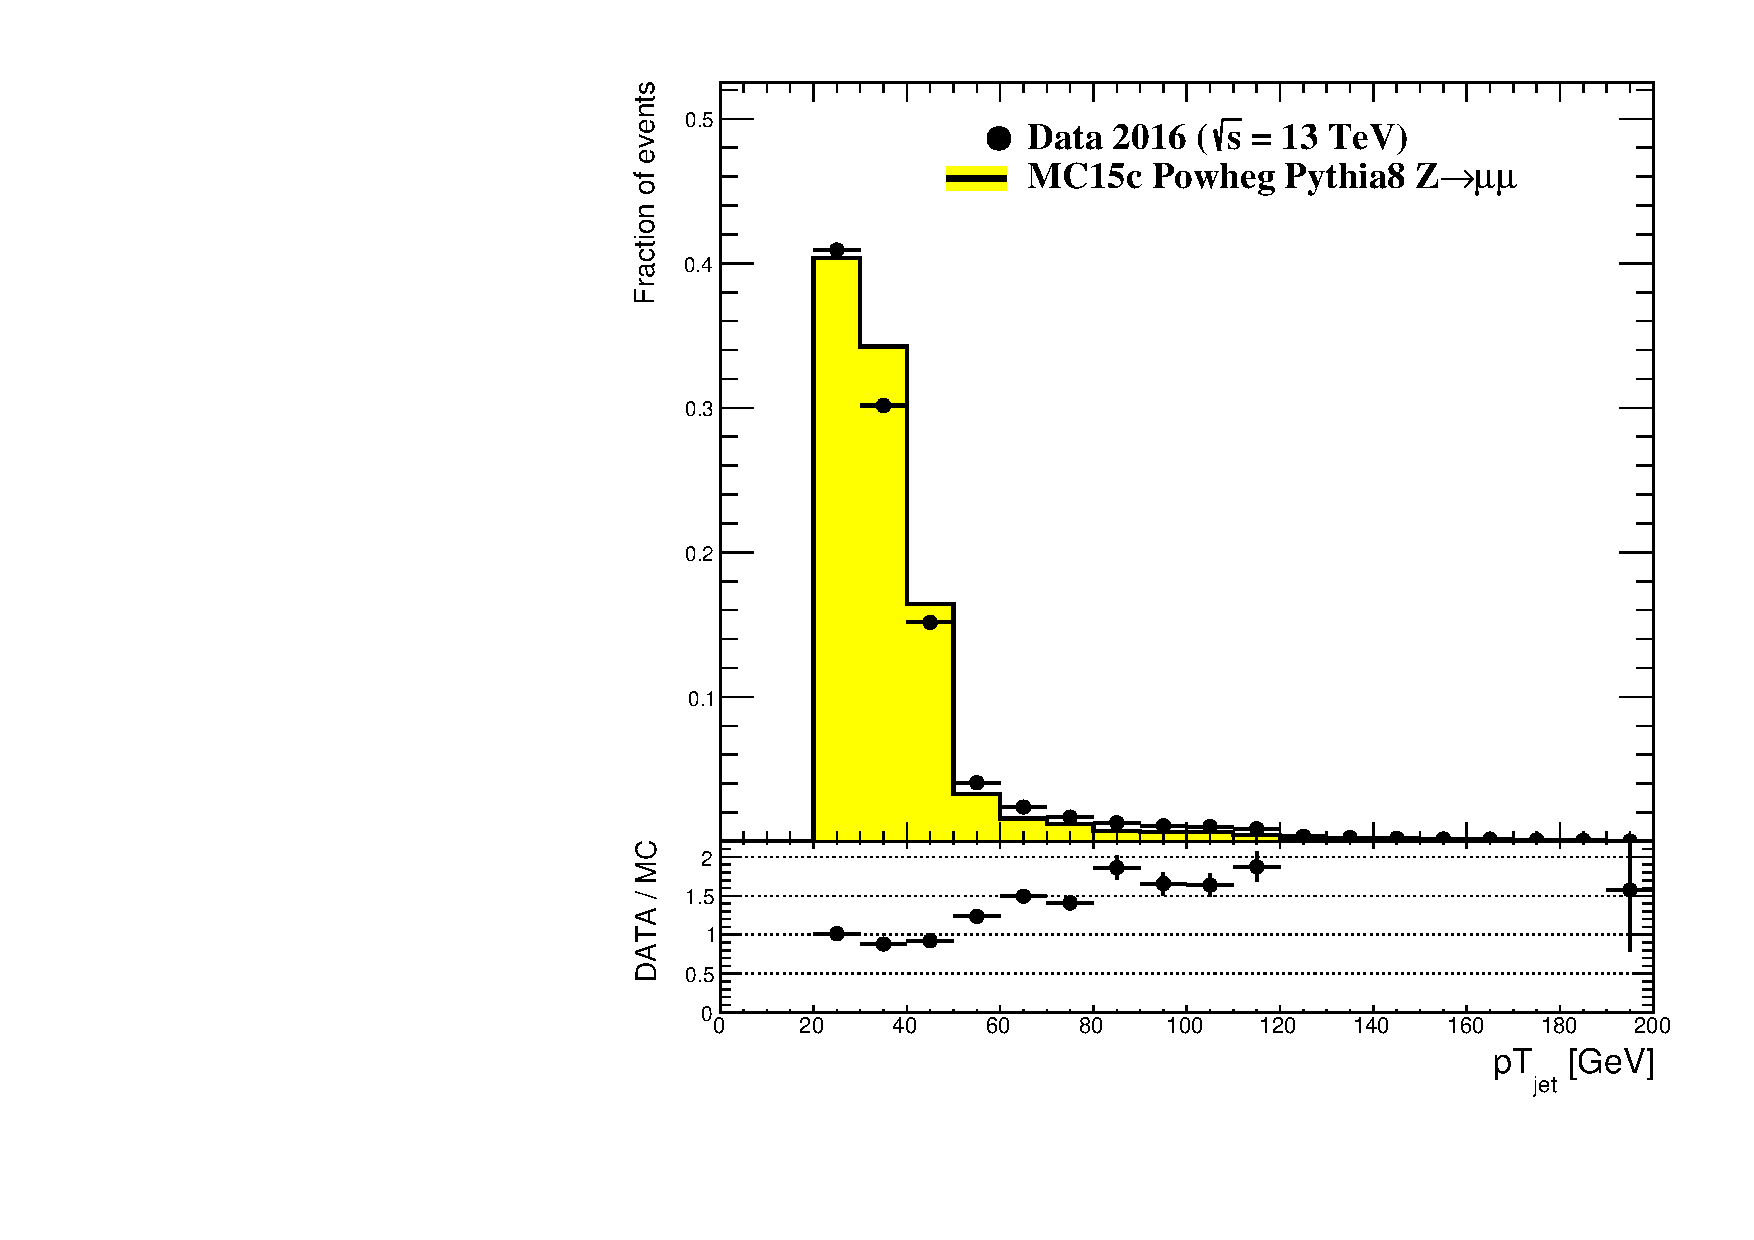
\includegraphics[width=0.53\figwidth]{jet_ptratio}
\caption[Transversal momentum of the recoiling jet]{$pT_{jet}$}
\label{fig:jetpt}
\end{subfigure}
\quad
\begin{subfigure}[b]{0.5\figwidth}
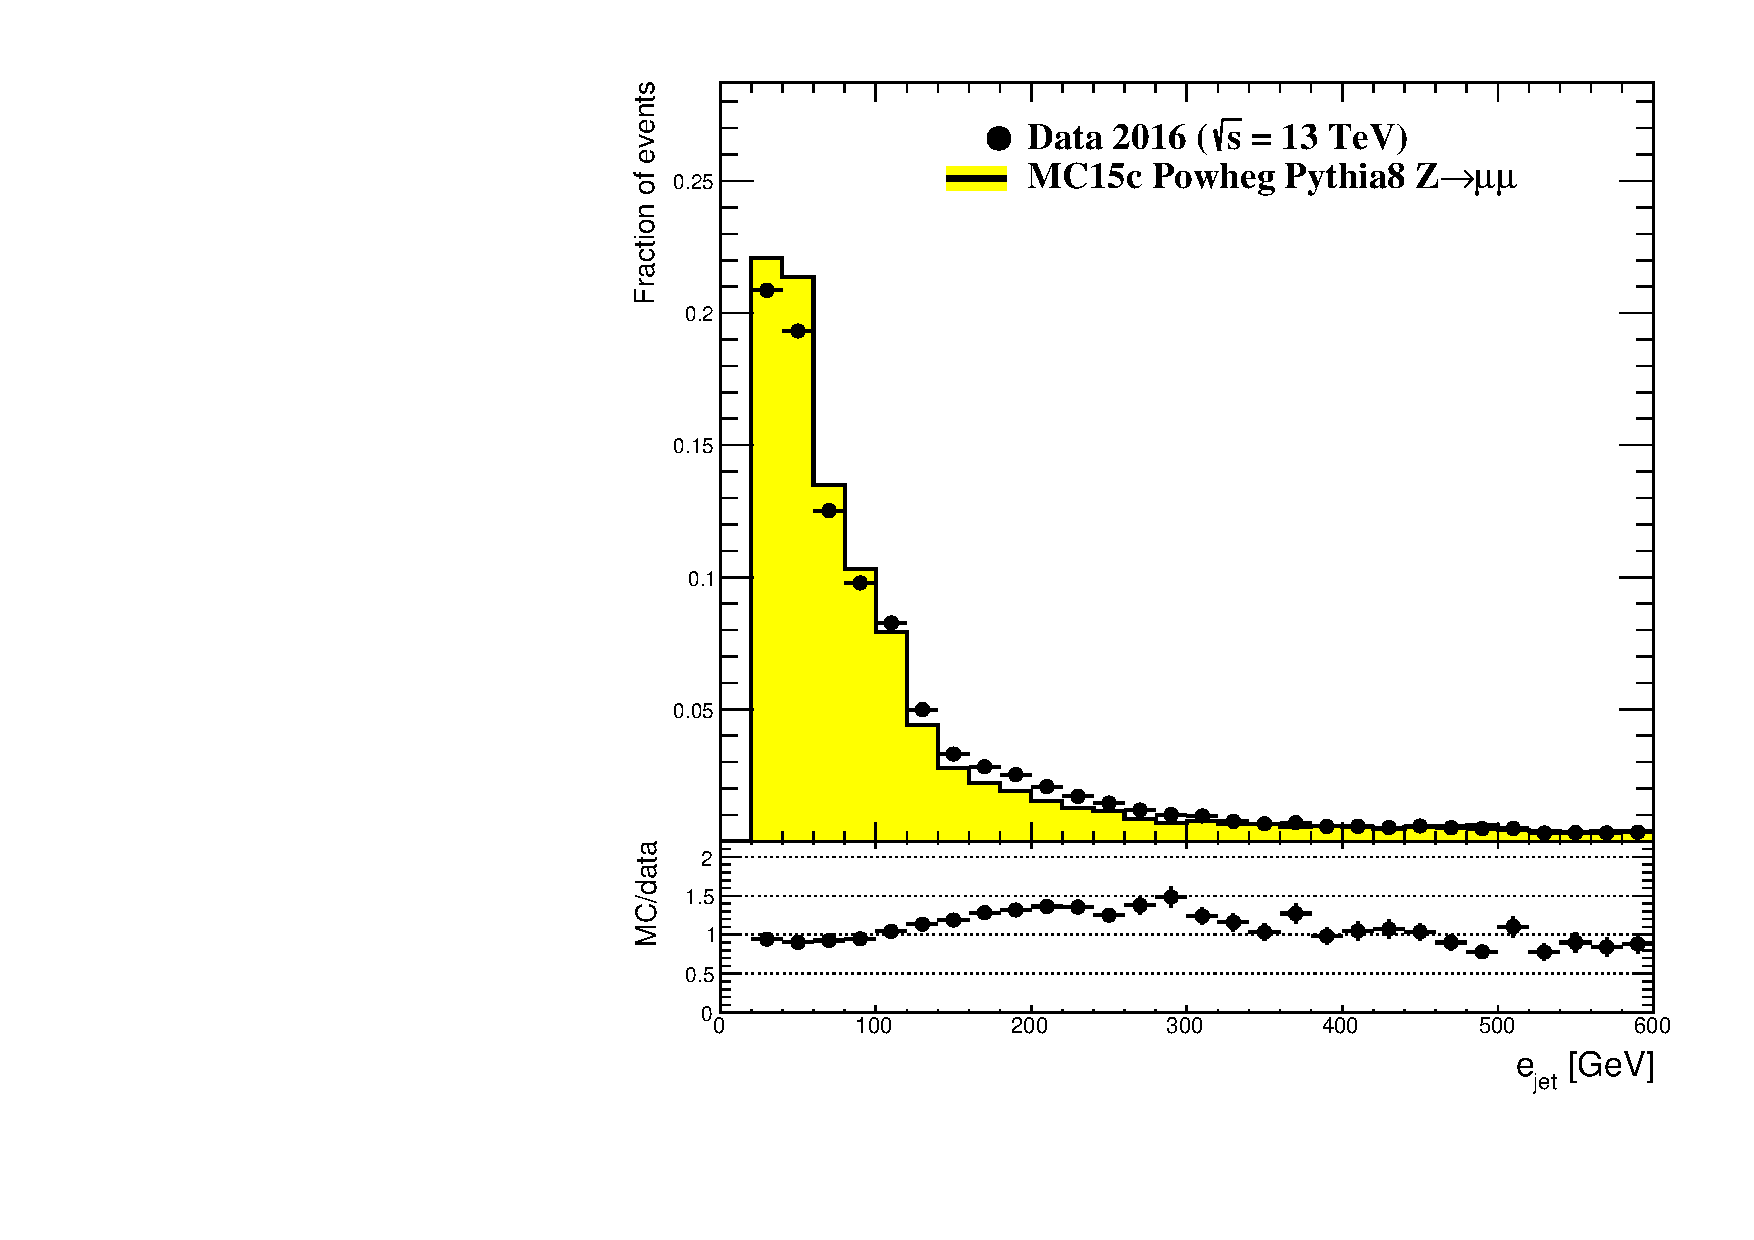
\includegraphics[width=0.53\figwidth]{jet_eratio}
\caption[Energy of the recoiling jet]{$e_{jet}$}
\label{fig:jete}
\end{subfigure}
\end{figure}


\begin{figure}[h]
\centering
\begin{subfigure}[b]{0.5\figwidth}
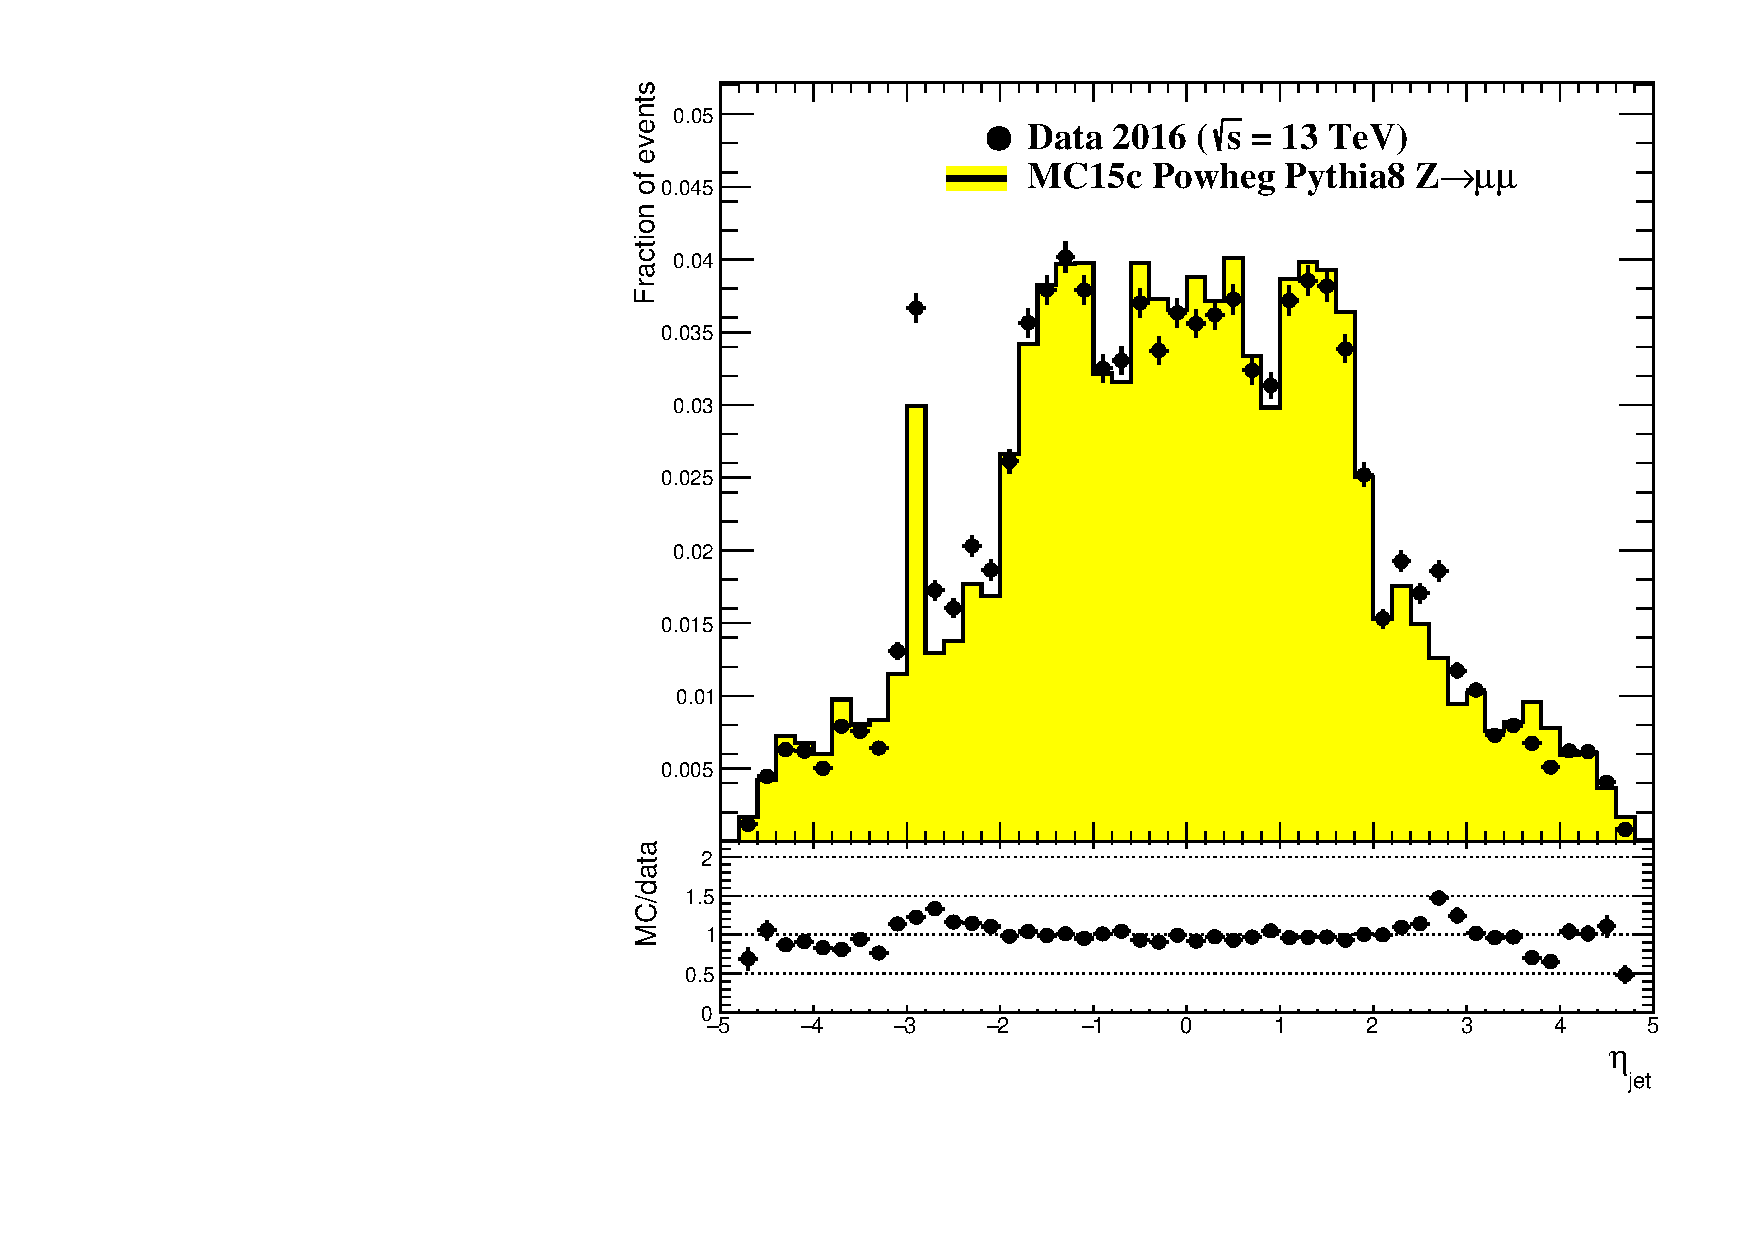
\includegraphics[width=0.53\figwidth]{jet_etaratio}
\caption[$\eta$ of the recoiling jet]{$\eta_{jet}$}
\label{fig:jeteta}
\end{subfigure}
\quad
\begin{subfigure}[b]{0.5\figwidth}
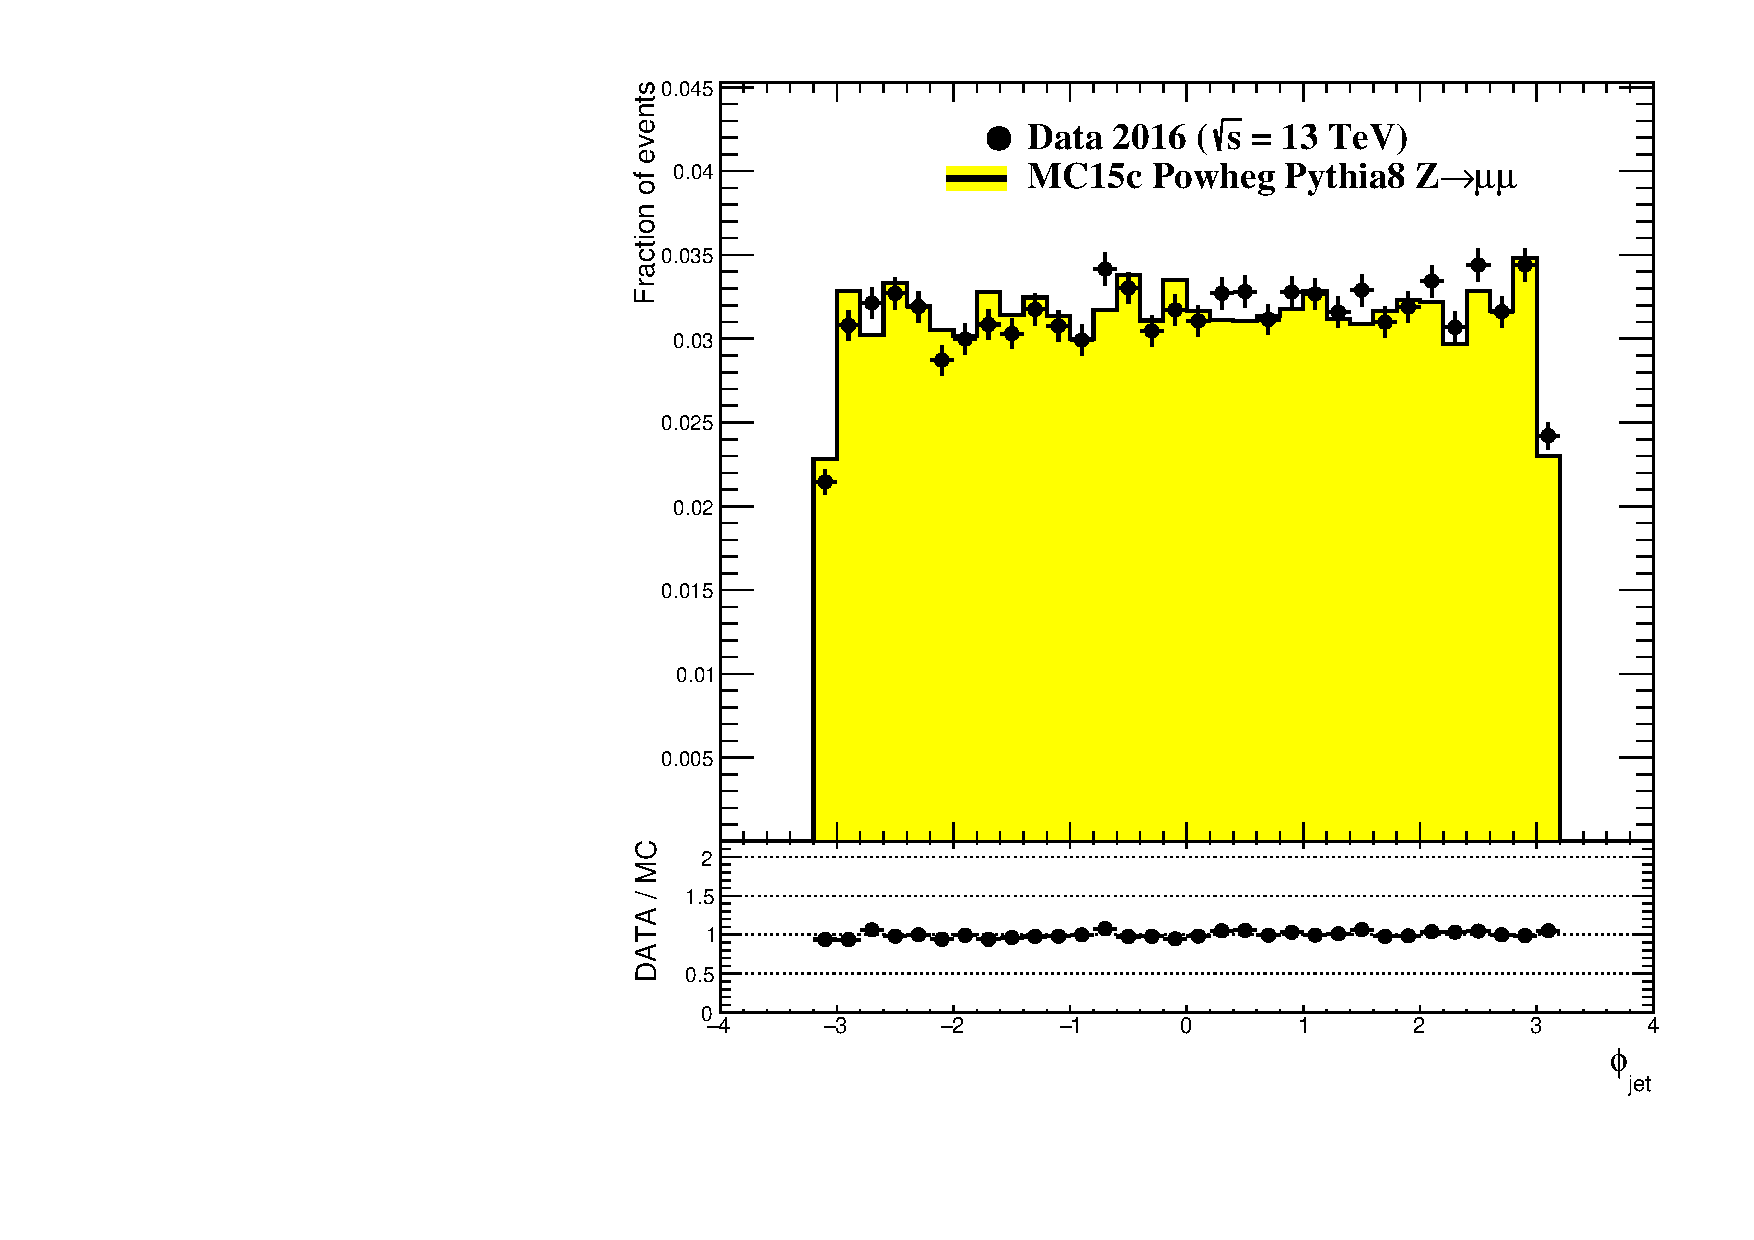
\includegraphics[width=0.53\figwidth]{jet_phiratio}
\caption[$\phi$ of the recoiling jet]{$\phi_{jet}$}
\label{fig:jetphi}
\end{subfigure}
\caption{Properties of the recoiling jet. The distributions are normalized to the number of jets. Distributions shown are: \ref{fig:jetpt} the jet's transversal momentum; \ref{fig:jete} the jet's energy; \ref{fig:jeteta} the jet's eta and \ref{fig:jetphi} the jet's phi.}
\label{fig:reoilingjet}
\end{figure}

\section{Reconstruction of the Z-Boson}

The $Z-Boson$ is reconstructed as the vector-sum of the two muons in the selected event.
It is required to be in an range of \SI{90+-10}{\GeV} and to have a transversal momentum greater than \SI{30}{\GeV}.

Figure \ref{fig:z} shows the properties of the reconstructed $Z$-Boson in data/MC comparison. The agreement of data and Monte Carlo for the $Z$ is in general very good. The momentum resolution worsens slightly with $pT$ exceeding $\SI{80}{\GeV}$ but keeps a reasonable value. The mass of the $Z-Boson$ fluctuates in a range of about \SI{5}{\GeV} around the expected value of \SI{91.19}{\GeV} and has a good agreement with the MC.
The angular agreement is also very good.


\begin{figure}[h]
\centering
\begin{subfigure}[b]{0.5\figwidth}
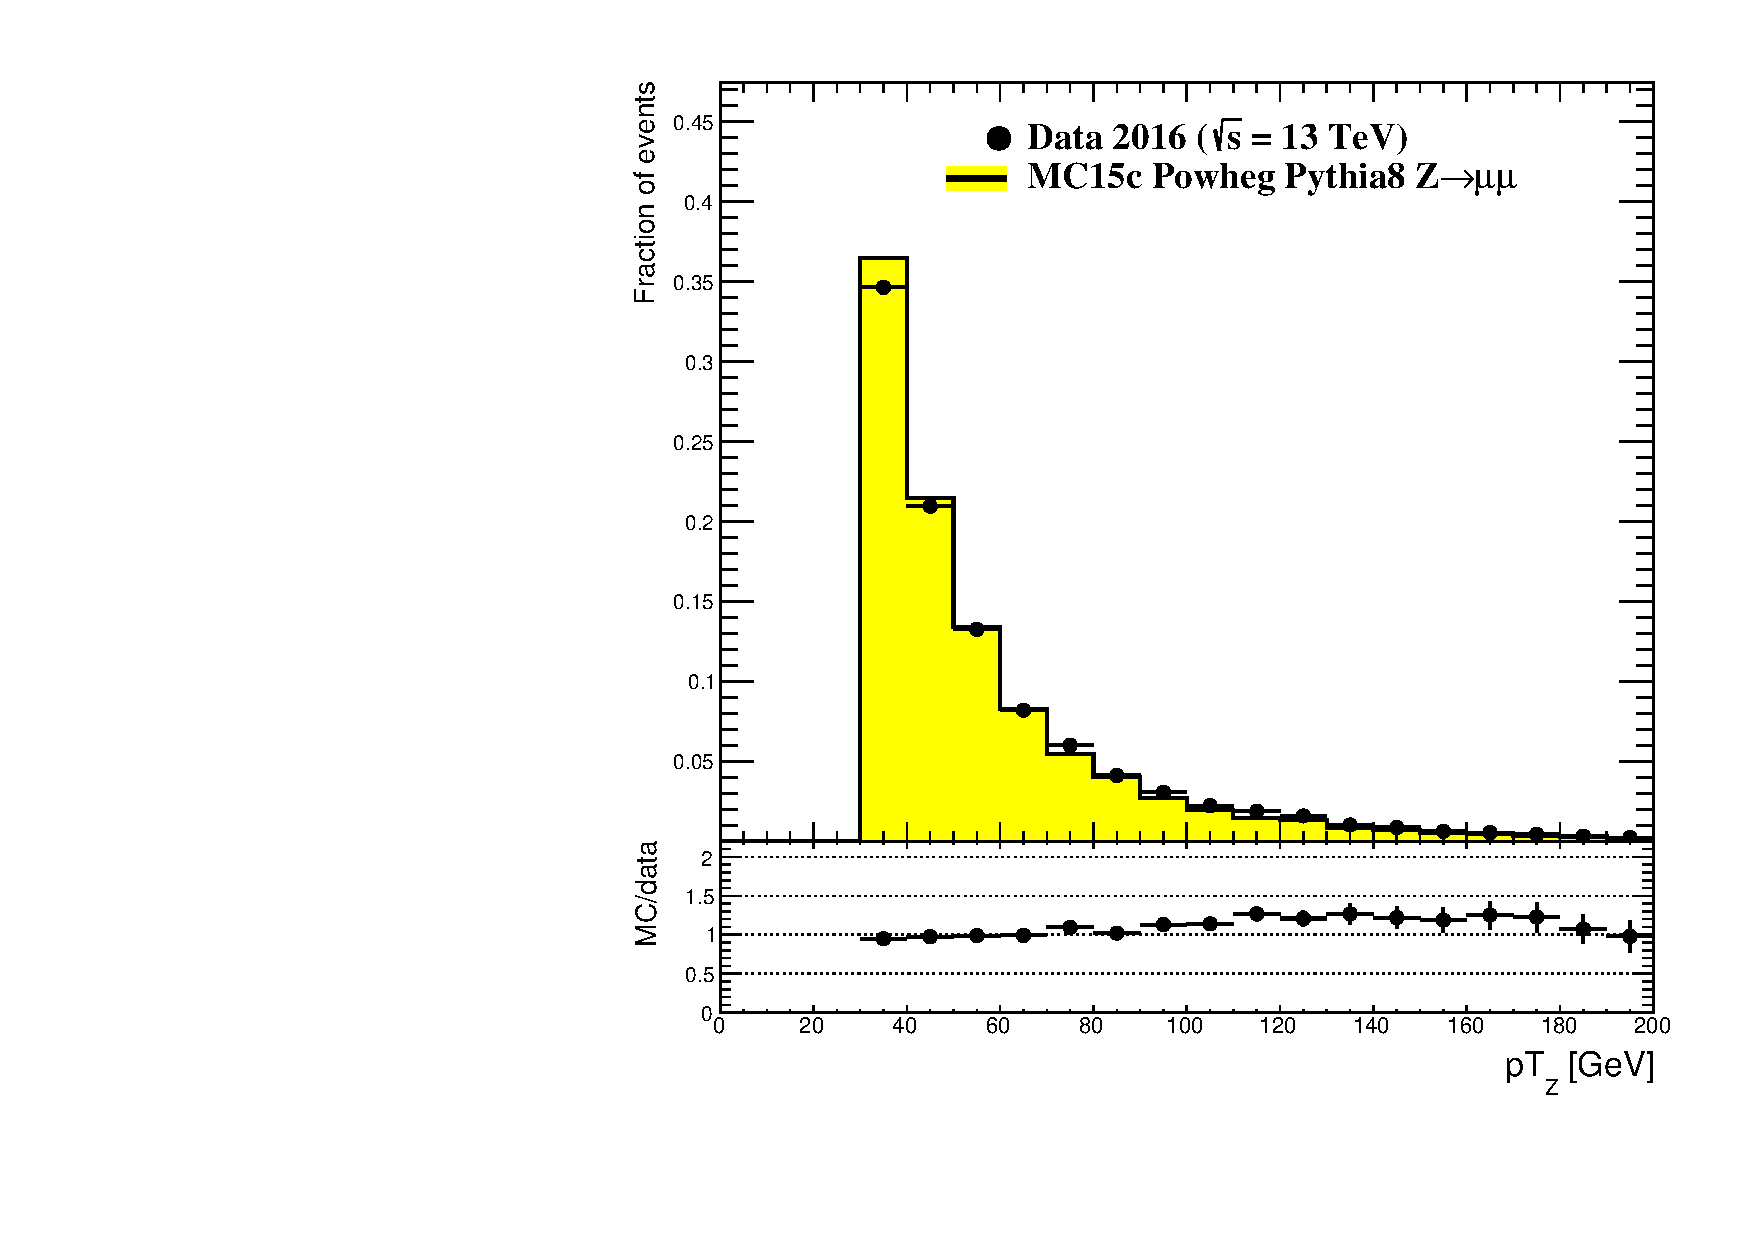
\includegraphics[width=0.53\figwidth]{Z_ptratio}
\caption[Transversal momentum of the reconstructed Z]{$pT_Z$}
\label{fig:zpt}
\end{subfigure}
\quad
\begin{subfigure}[b]{0.5\figwidth}
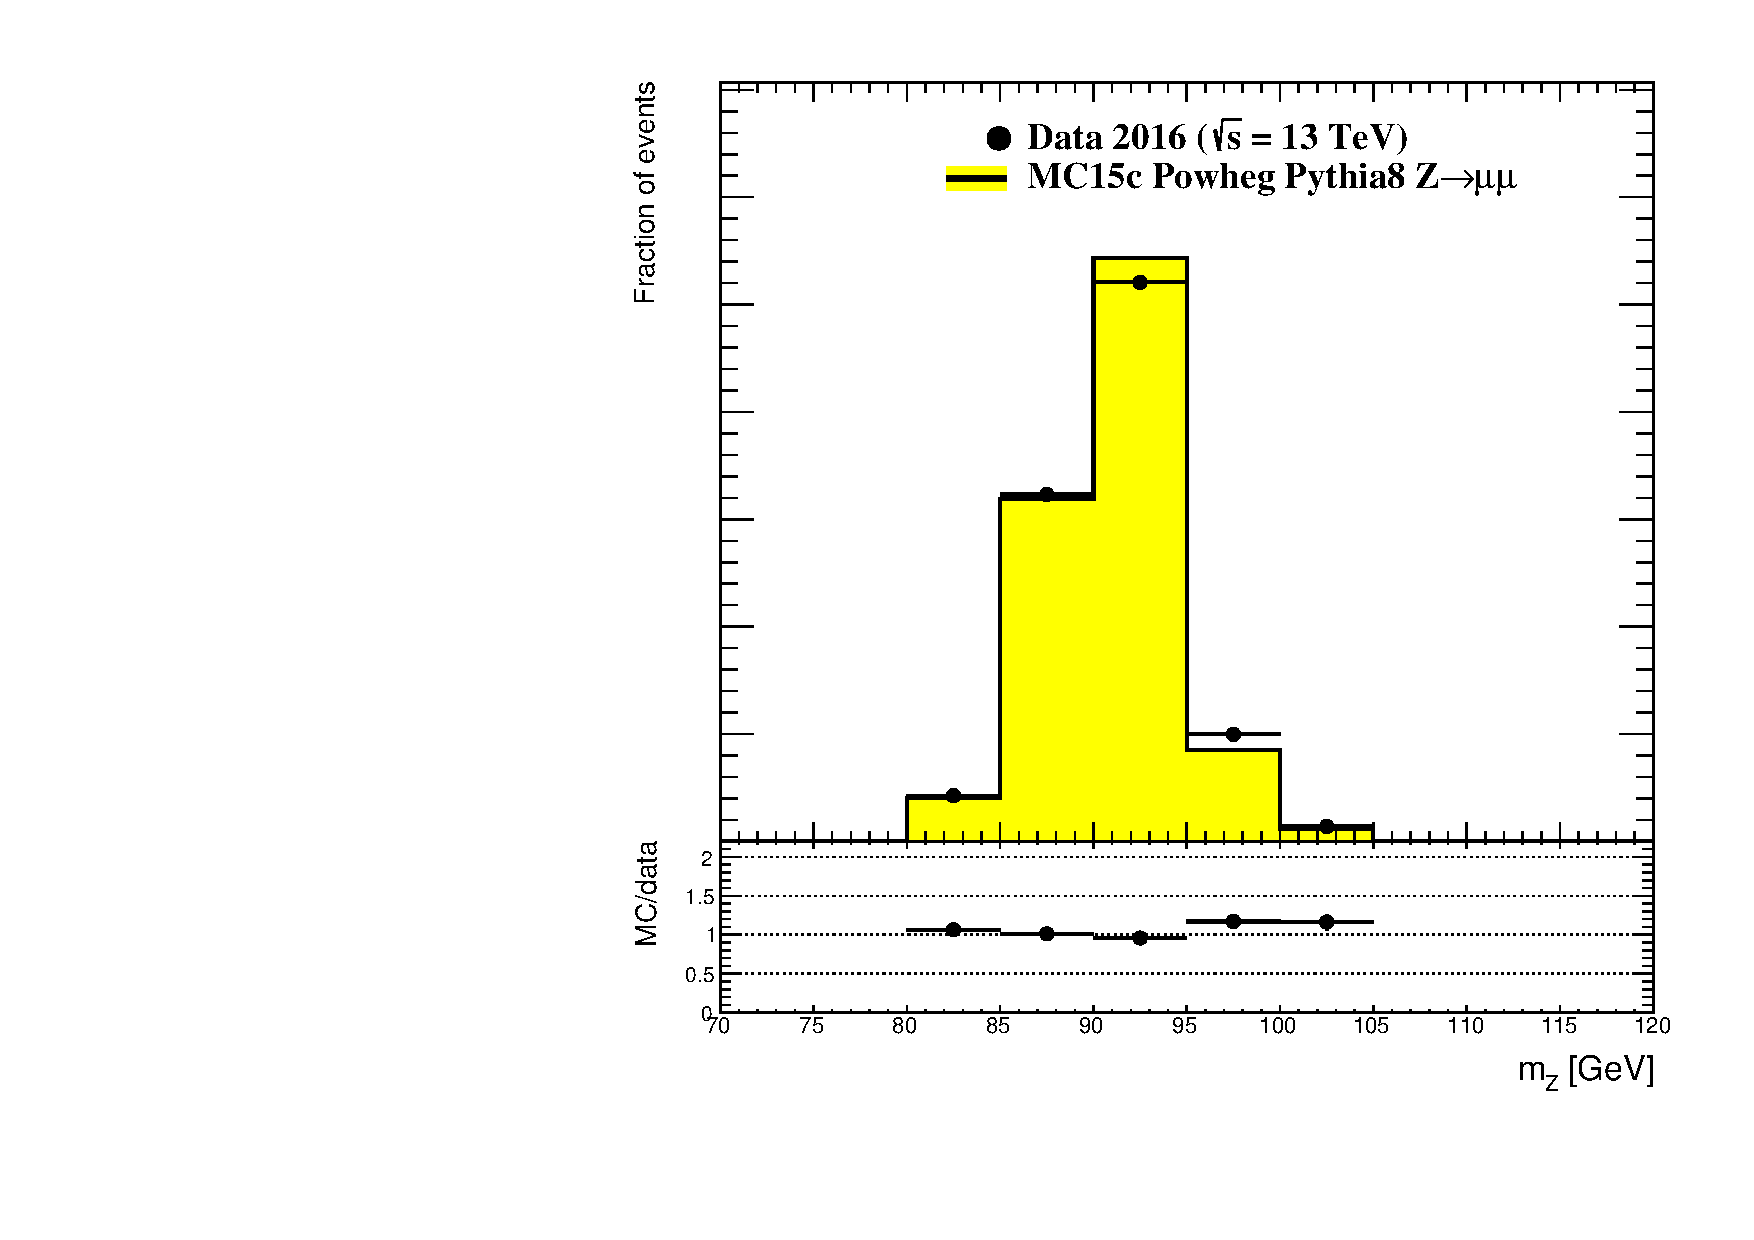
\includegraphics[width=0.53\figwidth]{Z_mratio}
\caption[mass of the reconstructed $Z$]{$m_Z$}
\label{fig:zm}
\end{subfigure}
\end{figure}


\begin{figure}[h]
\centering
\begin{subfigure}[b]{0.5\figwidth}
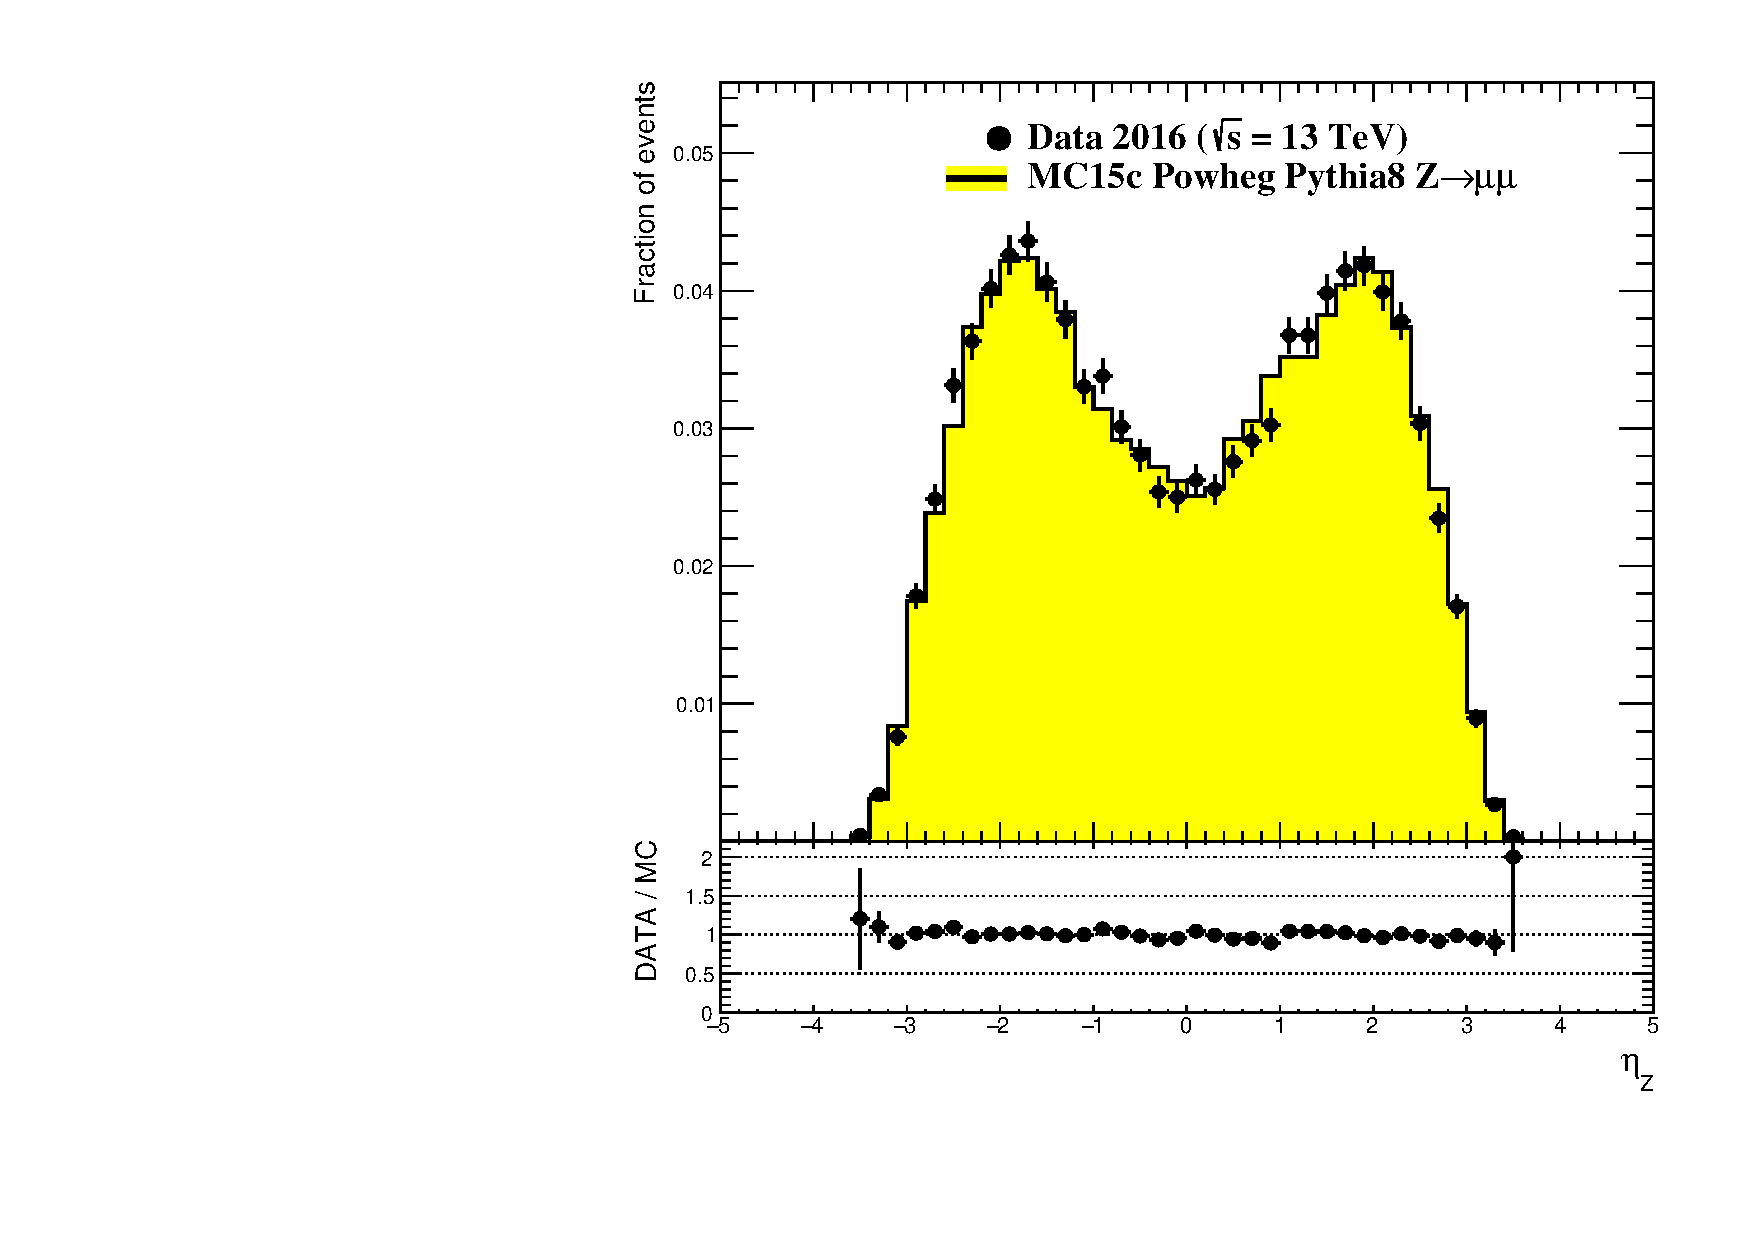
\includegraphics[width=0.53\figwidth]{Z_etaratio}
\caption[$\eta$ of the reconstructed $Z$]{$\eta_Z$}
\label{fig:zeta}
\end{subfigure}
\quad
\begin{subfigure}[b]{0.5\figwidth}
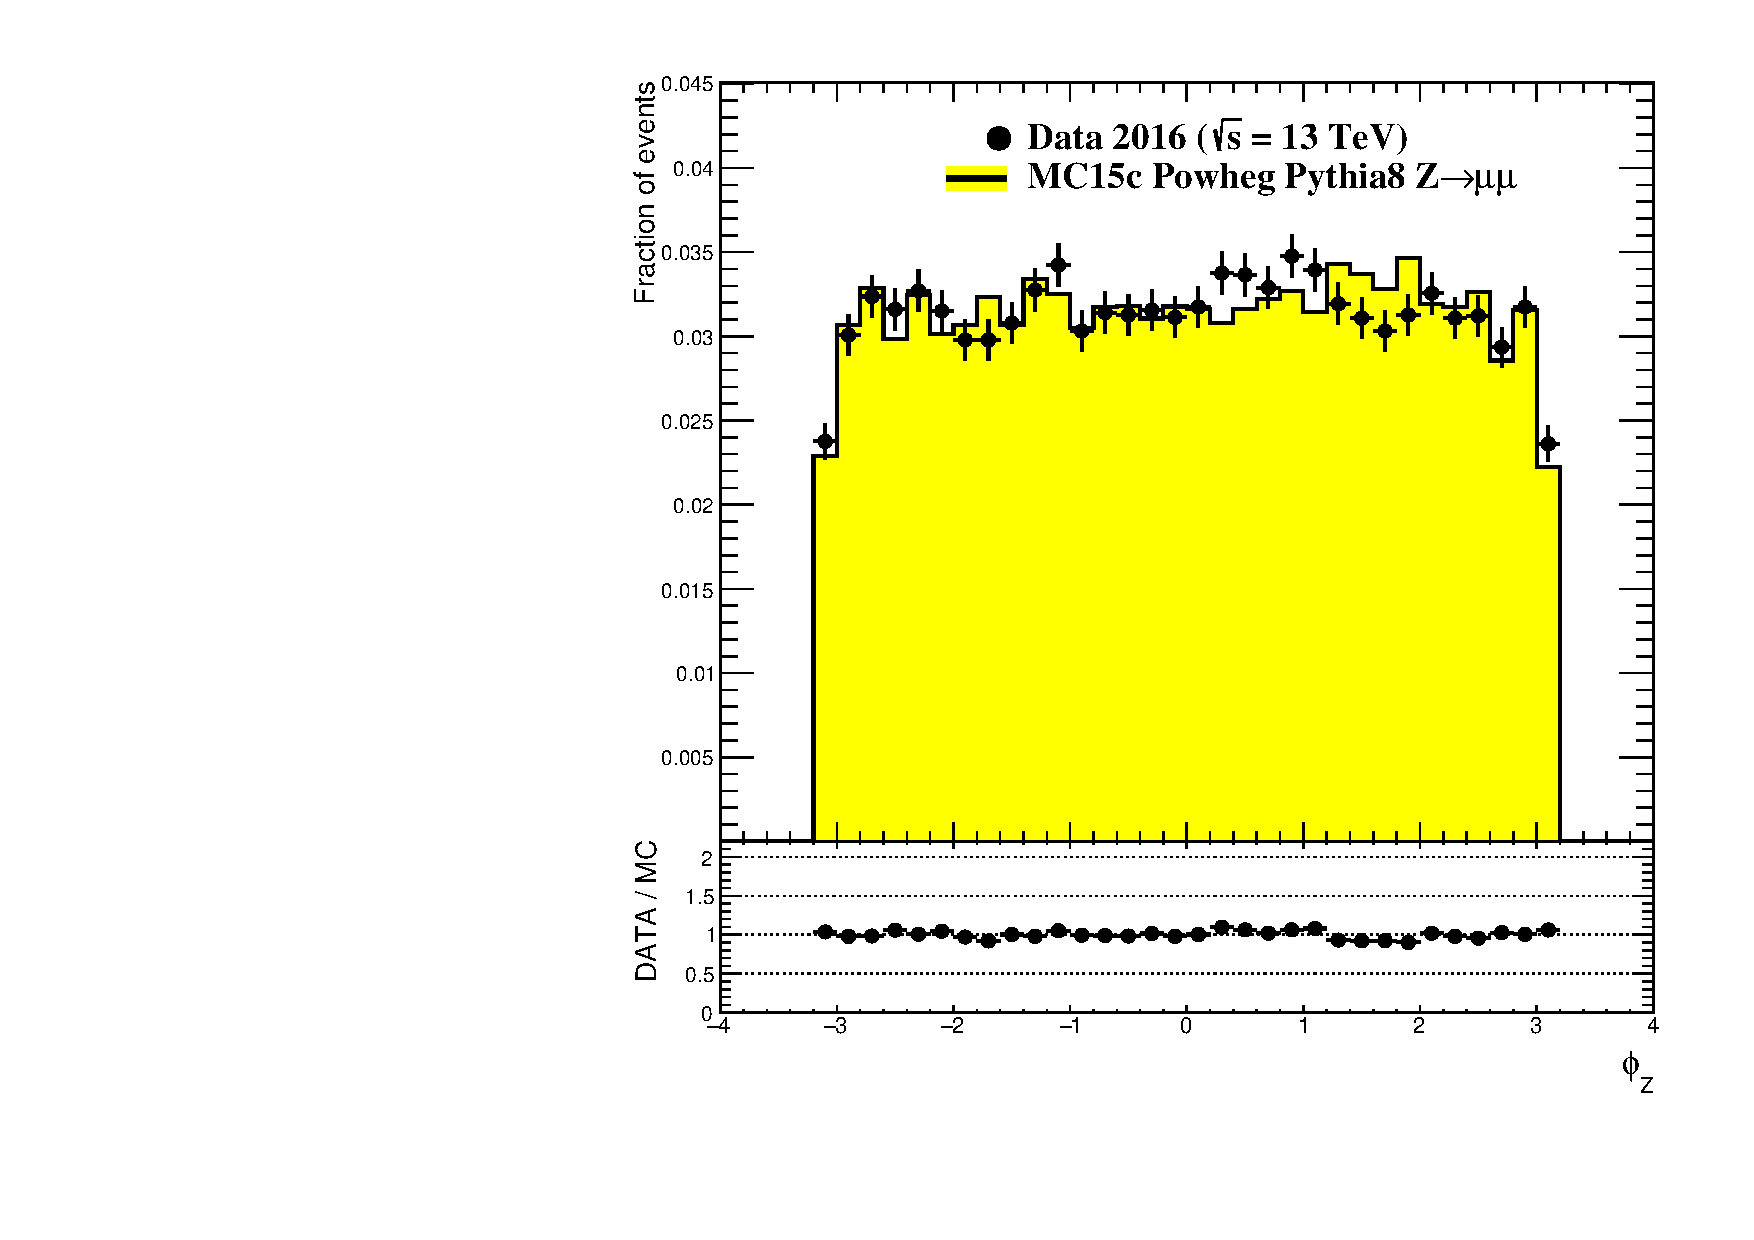
\includegraphics[width=0.53\figwidth]{Z_phiratio}
\caption[$\phi$ of the reconstructed $Z$]{$\phi_Z$}
\label{fig:zphi}
\end{subfigure}
\caption{Properties of the reconstructed Z-Boson. MC and data are normalized. The distributions show \ref{fig:zpt} the transversal momentum; \ref{fig:zm} the mass; \ref{fig:zeta} the pseudorapidity and \ref{fig:zphi} the $\phi$ of the $Z$.}
\label{fig:z}
\end{figure}



\section{Performance of general variables}


This sections shows the comparison of data and Monte Carlo for some further jet and event variables displayed in figure \ref{fig:generalproperties}.

The first distribution shows the number of vertices per event. The agreement between data and MC is rather bad. The center of the MC-distribution is displaced to the left with respect to the data distribution. This suggests that the MC needs further weighting to match the data better. Given that the completion of the weighting is still in process one can hope that a proper weighting of the vertices might also improve other distributions. Nevertheless the distributions for data and MC are comparable and show similar shapes.

The second distribution \ref{fig:chfrac} shows the fraction of jet-$pT$ carried by reconstructed tracks. The agreement is decent although a weighting in MC might optimize it still. The first bin here is not an overflow bin but refers to neutral objects.

The third distribution \ref{fig:trackcount} shows the number of tracks in a jet. The agreement worsens for a high track multiplicity. This might be due to insufficient statistics. Furthermore there might be wrong tracks reconstructed in data because the data multiplicity generally is higher that in MC.

The last distribution \ref{fig:trackwidth} shows the track width. The agreement is reasonable although the fluctuations can hopefully be mediated by further scaling.

\begin{figure}[h]
\centering
\begin{subfigure}[b]{0.5\figwidth}
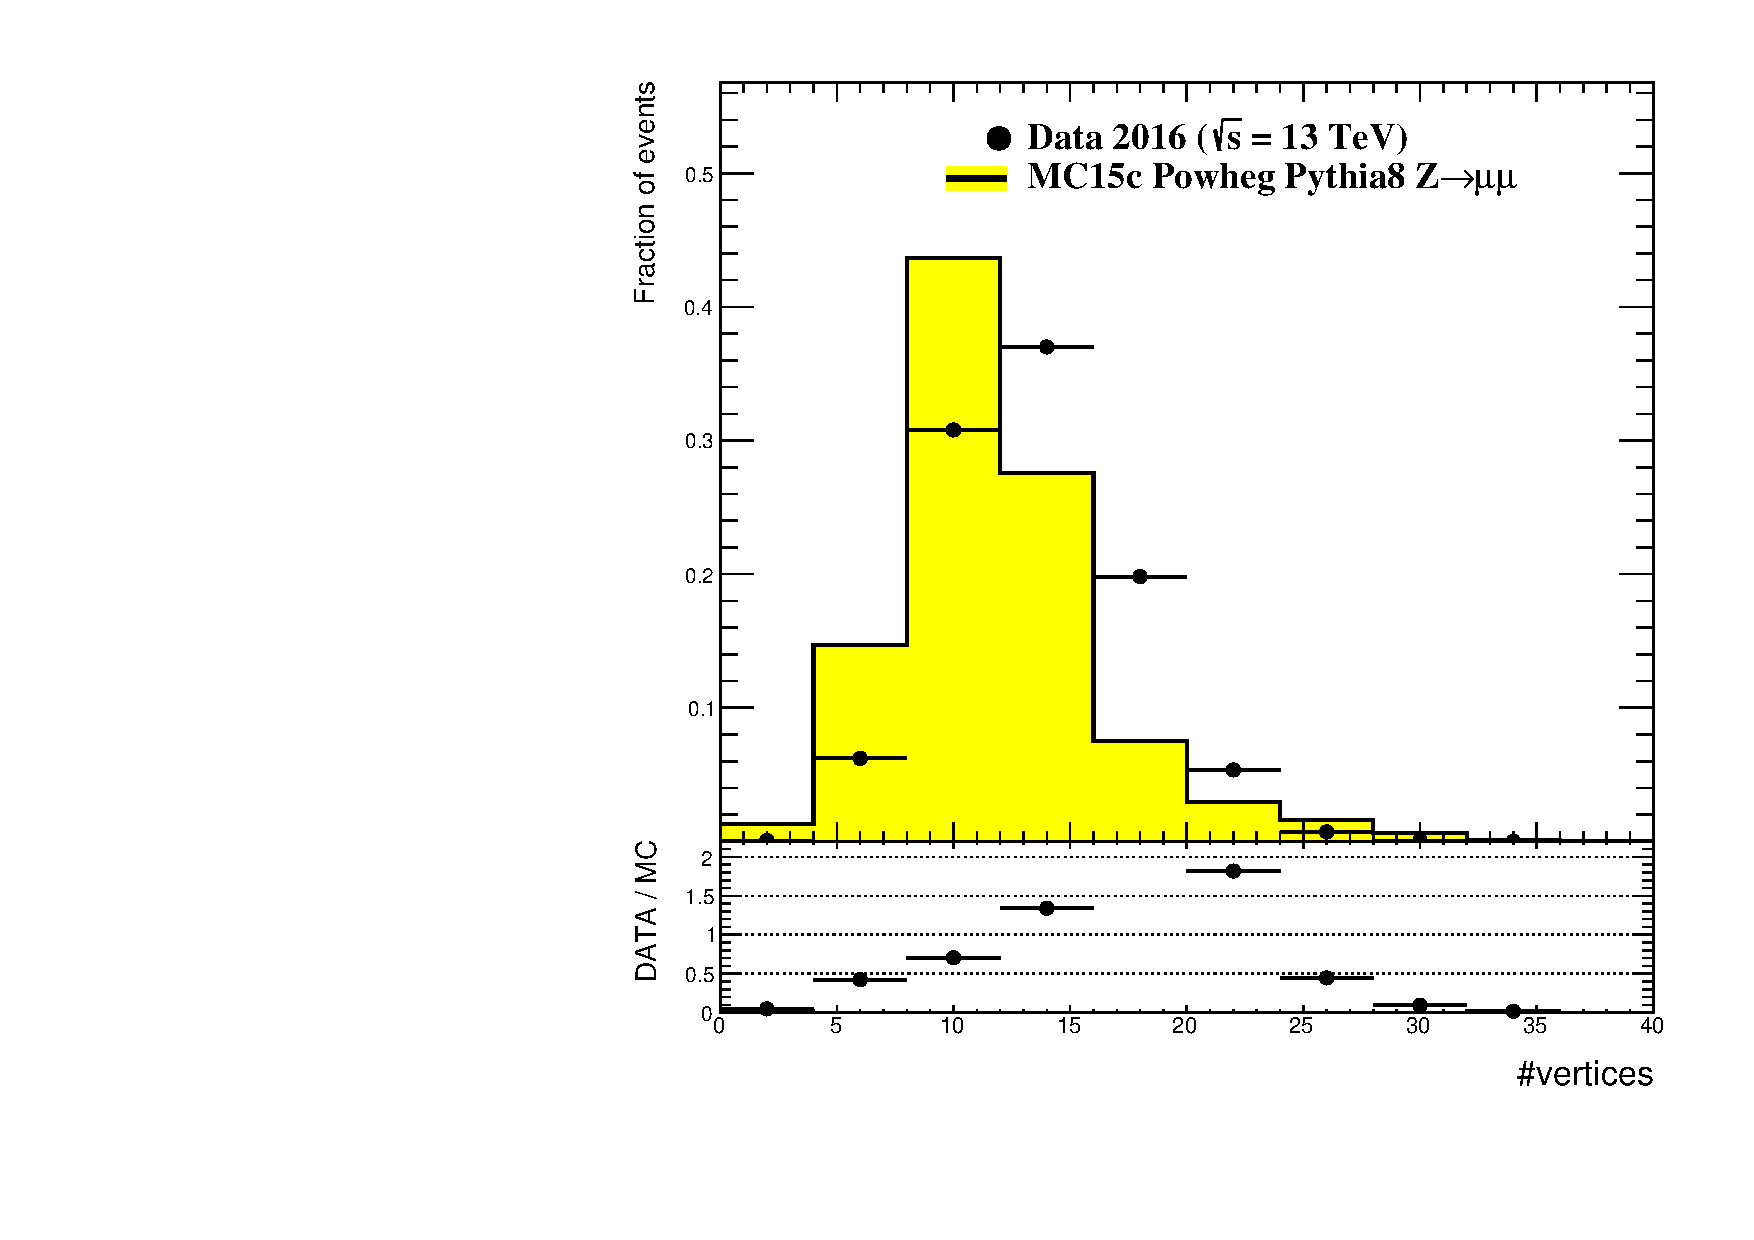
\includegraphics[width=0.53\figwidth]{verticesratio}
\caption[Number of vertices]{Number of vertices}
\label{fig:vertices}
\end{subfigure}
\quad
\begin{subfigure}[b]{0.5\figwidth}
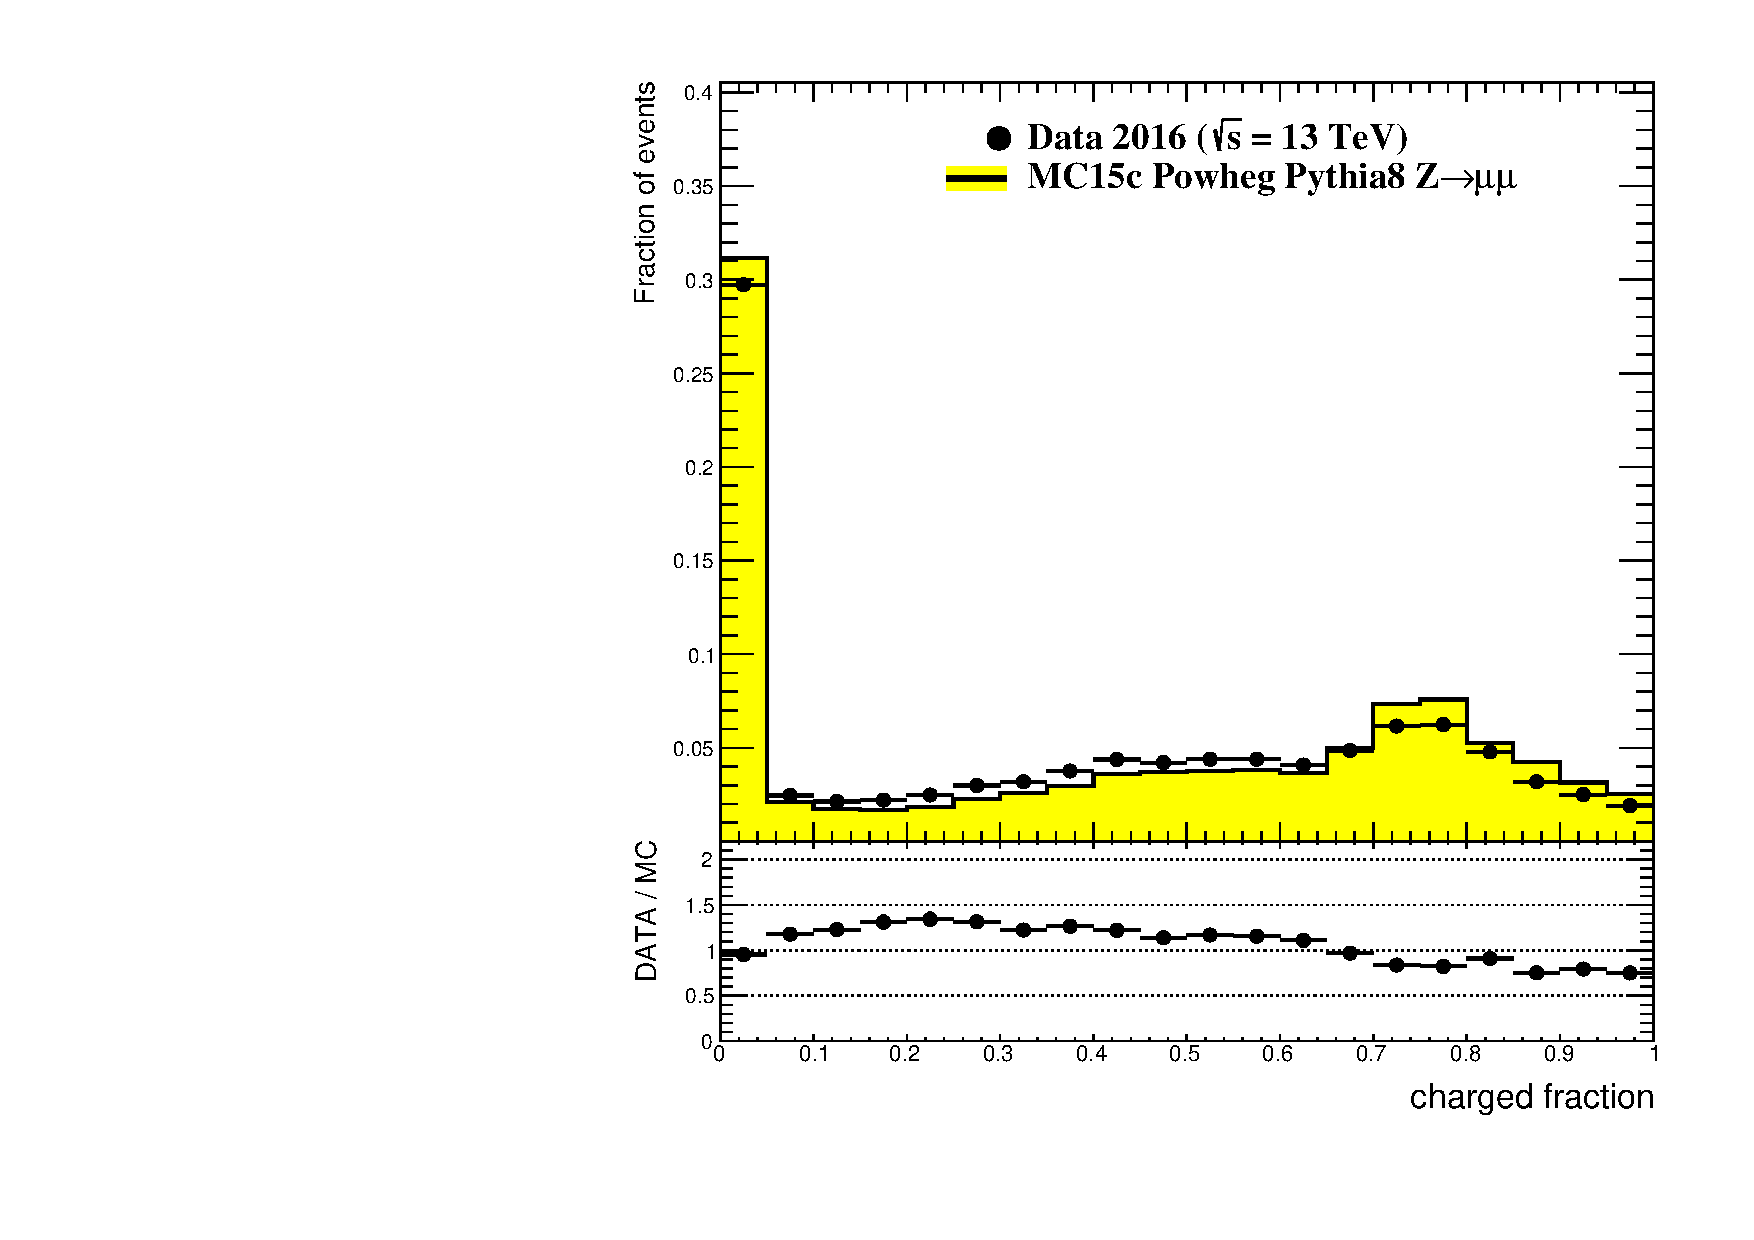
\includegraphics[width=0.53\figwidth]{chfracratio}
\caption[Charged fraction]{Charged fraction}
\label{fig:chfrac}
\end{subfigure}
\end{figure}


\begin{figure}[h]
\centering
\begin{subfigure}[b]{0.5\figwidth}
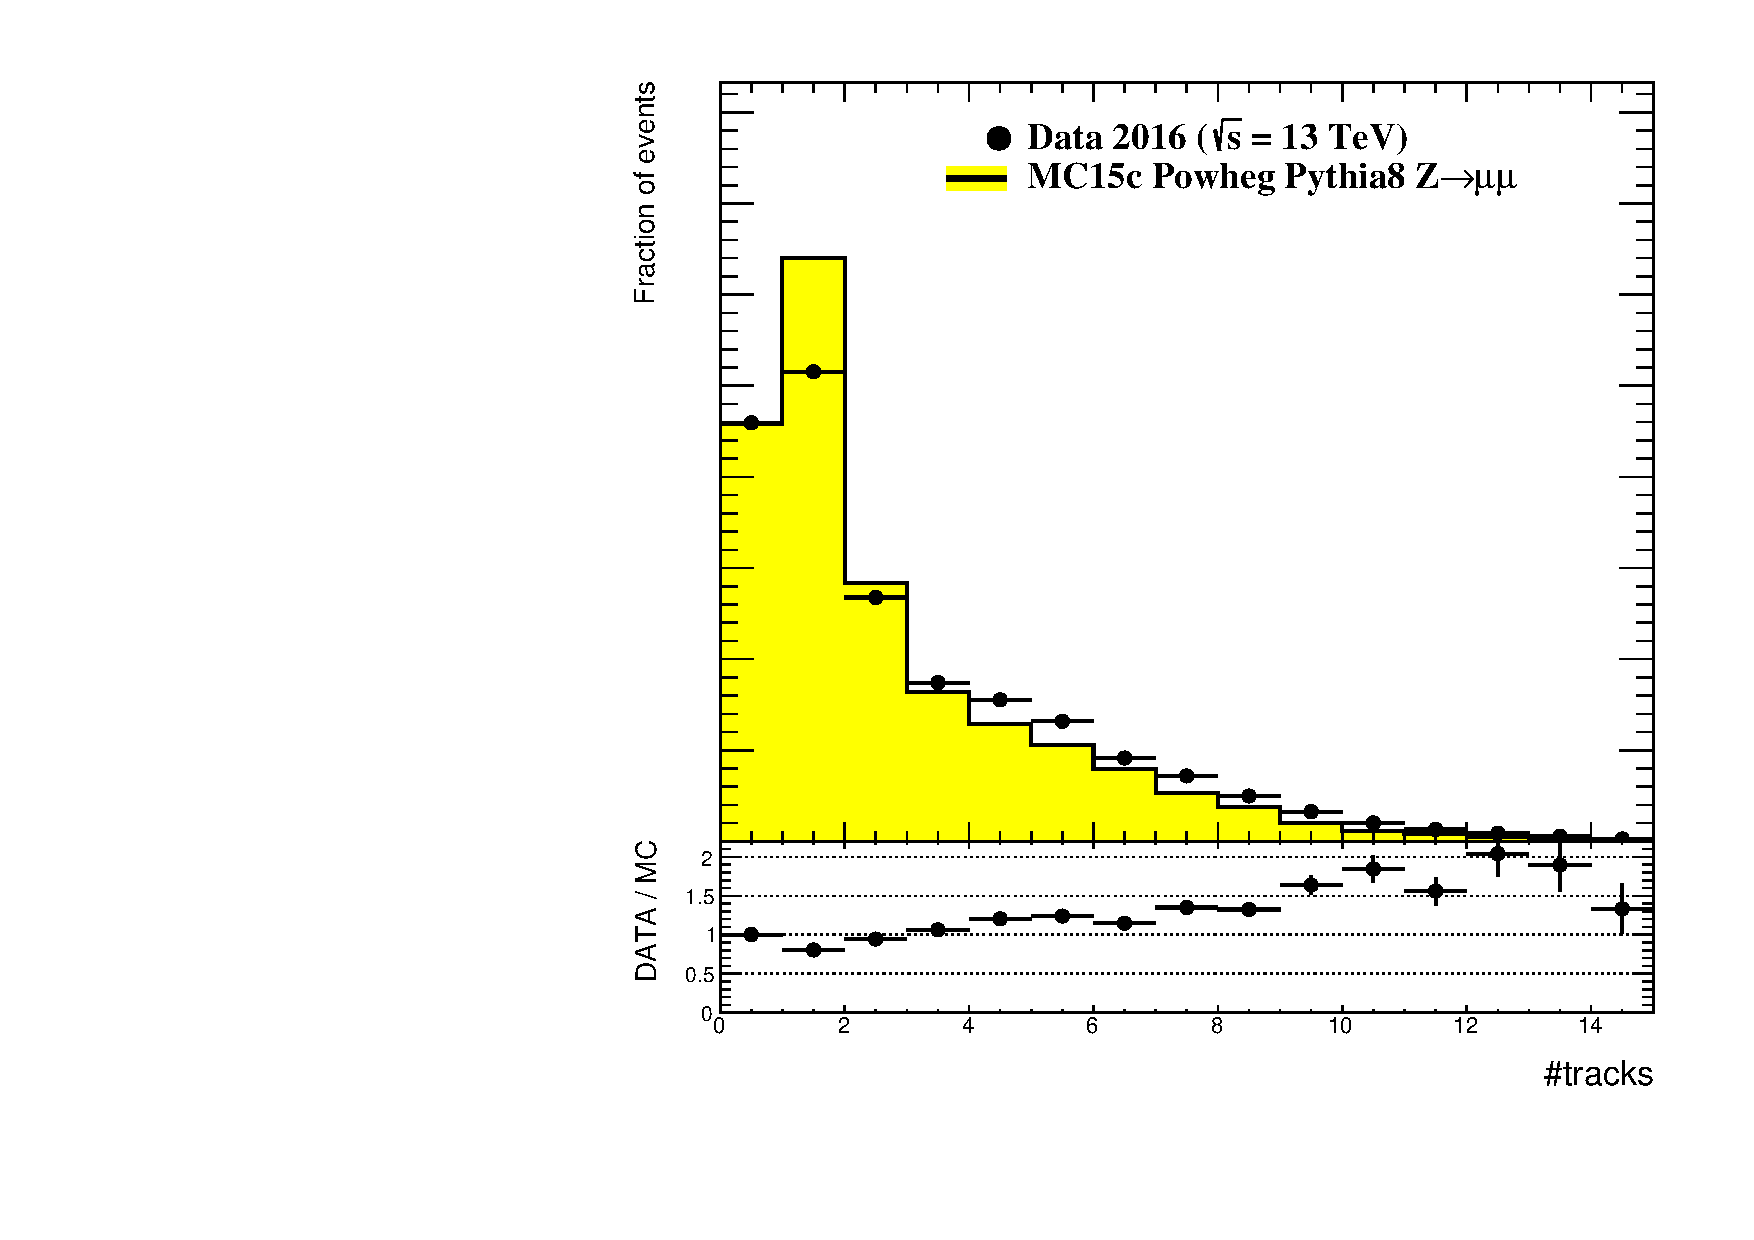
\includegraphics[width=0.53\figwidth]{trackcountratio}
\caption[Track count]{Track count}
\label{fig:trackcount}
\end{subfigure}
\quad
\begin{subfigure}[b]{0.5\figwidth}
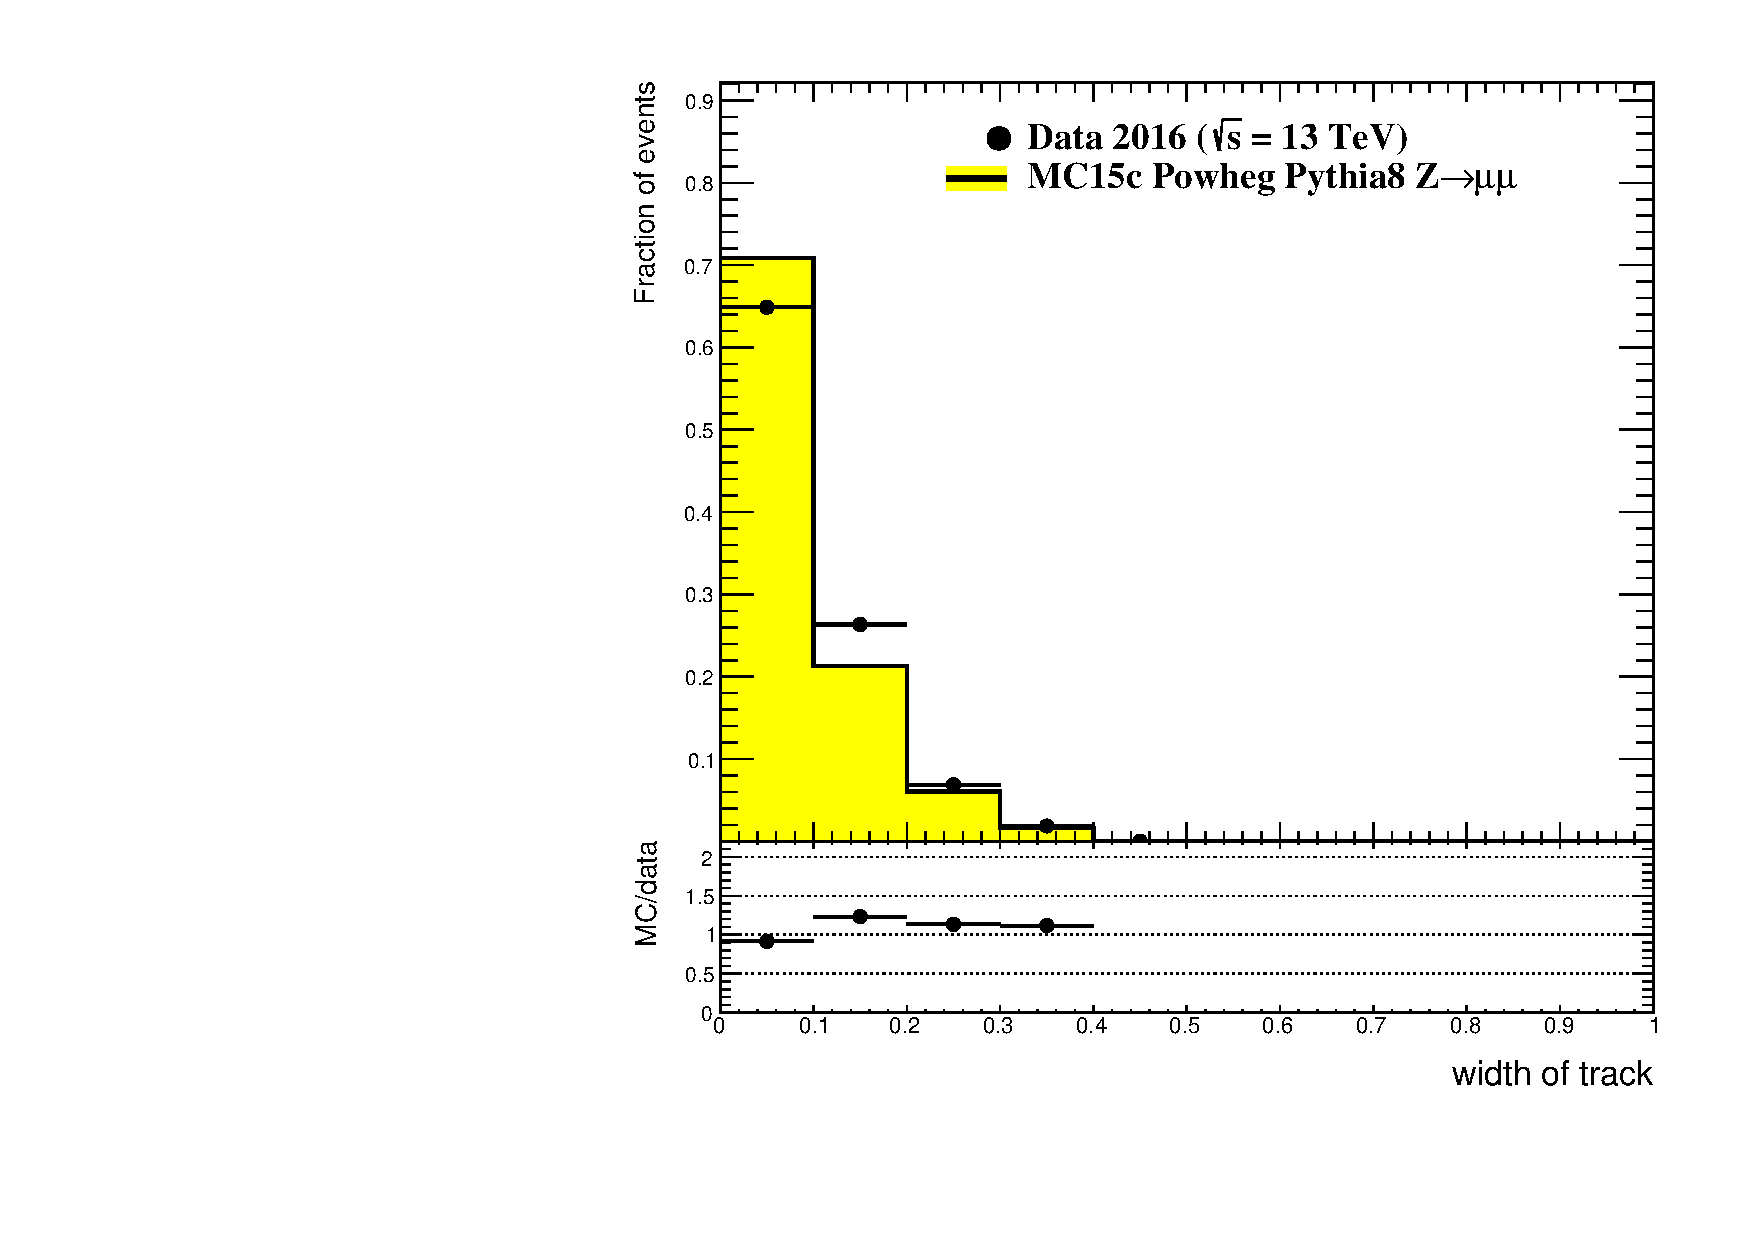
\includegraphics[width=0.53\figwidth]{trackwidthratio}
\caption[trackwidth]{Track width}
\label{fig:trackwidth}
\end{subfigure}
\caption{General event properties in data/MC comparison. The distributions are normalized to the sample size. The following distributions are shown: \ref{fig:vertices} number of vertices in the event; \ref{fig:chfrac} the charged fraction, i.e. the fractional jet $p_T$ carried by reconstructed tracks; \ref{fig:trackcount} the number of tracks in the jet; \ref{fig:trackwidth} the track's width.}
\label{fig:generalproperties}
\end{figure}


\section{Conclusion of the performance}

All things considered the data/MC comparison shows that the Particle Flow framework is on a good way. Right now a full jet calibration as well as jet cleaning for Particle Flow jets is missing. Furthermore the scale factors for all objects and further re-weighting for MC and data have to be applied.
With the improvements expected from these additional tools it is very likely that similar or better results as in Run 1 can be achieves using the Particle Flow algorithm.


\label{results}
